\documentclass[12pt,a4paper,openright]{book}

% Packages
\usepackage[utf8]{inputenc}
\usepackage[english]{babel}
\usepackage{amsmath,amsfonts,amssymb}
\usepackage{graphicx}
\usepackage{booktabs}
\usepackage{array}
\usepackage{float}
\usepackage{listings}
\usepackage{xcolor}
\usepackage{hyperref}
\usepackage{geometry}
\usepackage{fancyhdr}
\usepackage{titlesec}
\usepackage{algorithm}
\usepackage{algorithmic}
\usepackage{tikz}
\usepackage{pgfplots}
\usepackage{subcaption}

% Page setup
\geometry{margin=2.5cm}
\setlength{\headheight}{27.05pt}
\pagestyle{fancy}
\fancyhf{}
\fancyhead[LE,RO]{\thepage}
\fancyhead[LO]{\rightmark}
\fancyhead[RE]{\leftmark}

% Title formatting
\titleformat{\chapter}[display]
{\normalfont\huge\bfseries}{\chaptertitlename\ \thechapter}{20pt}{\Huge}

% Code styling
\lstset{
    language=Python,
    basicstyle=\ttfamily\small,
    keywordstyle=\color{blue},
    commentstyle=\color{gray},
    stringstyle=\color{red},
    numbers=left,
    numberstyle=\tiny,
    frame=single,
    breaklines=true,
    tabsize=4
}

% Hyperref setup
\hypersetup{
    colorlinks=true,
    linkcolor=blue,
    filecolor=magenta,
    urlcolor=cyan,
    pdftitle={Genetic Algorithms: Theory and Practice},
    pdfauthor={Course Materials},
    pdfsubject={Genetic Algorithms},
    pdfkeywords={genetic algorithms, optimization, evolutionary computation}
}

% TikZ libraries
\usetikzlibrary{shapes,arrows,positioning,calc}

% Title page information
\title{
    \Huge\textbf{Genetic Algorithms}\\
    \Large\textit{Theory and Practice}\\
    \vspace{1cm}
    \large A Comprehensive Guide to Evolutionary Optimization
}
\author{Course Materials Collection}
\date{\today}

\begin{document}

% Title page
\frontmatter
\maketitle

% Table of contents
\tableofcontents
\listoffigures
\listoftables

% Main content
\mainmatter

% Include chapters
\chapter{Introduction to Optimization and Evolutionary Computation}

  Genetic algorithms (GAs) are population-based search methods inspired by natural selection and genetics. They maintain a population of candidate solutions encoded as strings, iteratively producing new generations by selecting the fittest individuals, recombining their information, and occasionally introducing random variation. Although stochastic in their operators, GAs are not blind random walks: they retain and exploit historical information about good solutions to generate promising new search points and thereby drive efficient exploration and exploitation of complex spaces.

  This family of methods was developed from foundational work by Holland and colleagues to both model adaptive processes observed in nature and to design artificial systems that embody those mechanisms. A central aim has been robustness—the ability to balance efficiency with reliability across a wide range of problem environments—which makes GAs attractive when redesign costs are high or when problem structure violates common assumptions (e.g., continuity, differentiability, or unimodality). Because they are conceptually simple, widely applicable, and empirically effective in optimization and control, genetic algorithms have become a practical tool across engineering, science, and business domains \cite{goldberg1989genetic}.

  To place genetic algorithms in context, we first give a concise definition of optimization — the class of problems GAs are commonly used to solve.
    We define optimization as the process of finding the best solution from a set of available alternatives. In mathematical terms, an optimization problem can be formulated as:

  \begin{equation}
  \begin{aligned}
  \text{minimize (or maximize)} \quad & f(x) \\
  \text{subject to} \quad & g_i(x) \leq 0, \quad i = 1, 2, \ldots, m \\
  & h_j(x) = 0, \quad j = 1, 2, \ldots, p \\
  & x \in X
  \end{aligned}
  \end{equation}

  where:
  \begin{itemize}
      \item $f(x)$ is the objective function to be optimized
      \item $g_i(x)$ are inequality constraints
      \item $h_j(x)$ are equality constraints
      \item $X$ is the feasible region
  \end{itemize}

    Optimization problems differ by variable types (discrete, continuous, or mixed-integer) and by structural properties such as linearity, convexity, and the number of objectives. 
    Traditional solution methods include gradient-based techniques (e.g., Newton and quasi-Newton methods) for smooth continuous problems, linear programming (Simplex and interior-point methods) for linear models, and discrete methods (branch-and-bound, dynamic programming) for combinatorial problems. 
    However, these traditional methods have limitations when applied to many complex real-world problems. In the following sections we highlight three key challenges where conventional approaches often struggle, and explain how genetic algorithms can help address them.


    The first problem with traditional optimization methods is their tendency to get trapped in local optima.
    In multi-modal landscapes with many peaks and valleys, gradient-based searches can converge to a local 
    optimum rather than the global optimum. This happens because these methods rely on local gradient 
    information to guide the search process. When the search reaches a local optimum, the gradient 
    becomes zero, causing the algorithm to stop progressing. This limitation is particularly 
    problematic in high-dimensional spaces where the number of local optima can grow exponentially.

  \begin{figure}[H]
    \centering
    \begin{tikzpicture}
    \begin{axis}[
      width=0.9\textwidth,
      height=5cm,
      scale only axis,
      ymin=-4,
      ymax=4,
      xlabel={$x$},
      ylabel={$f(x)$},
      title={Gradient Descent Getting Trapped in Local Minimum},
      grid=major,
      legend pos=north west,
    ]
    % Multi-modal function
    \addplot[blue, thick, domain=-5:5, samples=200] {sin(deg(x))*3 + 0.1*x^2 - 2};
    \addlegendentry{Objective Function}

    % Local minimum point
    \addplot[red, mark=*, mark size=3pt] coordinates {(-4.5, -1.8)};
    \node[red] at (axis cs:-4.5,-0.8) {Local Minimum (Trapped)};

    % Global minimum point
    \addplot[green!60!black, mark=*, mark size=3pt] coordinates {(1.5, -3.2)};
    \node[green!60!black] at (axis cs:1.5,-2.2) {Global Minimum};

    % Gradient descent path
    \addplot[red, thick, ->] coordinates {(-3.5, 0.5) (-4.2, -1.2) (-4.5, -1.8)};
    \node[red] at (axis cs:-3.5,1.2) {Gradient Path};
    \end{axis}
    \end{tikzpicture}
    \caption{Traditional gradient-based methods follow the local gradient and become trapped in local optima, unable to escape to find the global optimum.}
  \end{figure}

  The second problem with gradient-based methods is that they require the objective function to be differentiable. This becomes a significant limitation when dealing with real-world problems that involve discontinuities, sharp corners, or discrete jumps.
  Such problems are common in engineering design, scheduling, and combinatorial optimization.

  \begin{figure}[H]
  \centering
  \begin{tikzpicture}
  \begin{axis}[
      width=12cm,
      height=6cm,
      xlabel={$x$},
      ylabel={$f(x)$},
      title={Non-Differentiable Function Example},
      grid=major,
      ymin=-2,
      ymax=3,
  ]
  % Piecewise function with discontinuities
  \addplot[blue, thick, domain=-3:-0.5, samples=50] {x + 1};
  \addplot[blue, thick, domain=-0.5:0.5, samples=50] {-2*x};
  \addplot[blue, thick, domain=0.5:2, samples=50] {x^2 - 1};
  \addplot[blue, thick, domain=2:3, samples=50] {-x + 5};

  % Mark discontinuities
  \addplot[red, mark=*, mark size=3pt, only marks] coordinates {(-0.5, 0.5) (0.5, -1) (2, 3)};
  \node[red] at (axis cs:1, 2.5) {Non-differentiable points};
  \draw[red, dashed, ->] (axis cs:1, 2.3) -- (axis cs:0.5, -0.5);

  \node[blue] at (axis cs:-2, -1.5) {\textcolor{red}{\textbf{×}} Gradient-based methods fail};
  \end{axis}
  \end{tikzpicture}
  \caption{Functions with discontinuities, sharp corners, or discrete jumps cannot be optimized using gradient-based methods.}
  \end{figure}

  % \textbf{How GAs Address This:}
  % \begin{itemize}[leftmargin=*]
  %     \item \textbf{Derivative-free}: GAs only require the ability to evaluate the fitness function, not compute derivatives
  %     \item \textbf{Black-box optimization}: Can handle any function that can be evaluated, regardless of mathematical properties
  %     \item \textbf{Handles discontinuities}: Works equally well with continuous, discrete, or mixed-variable problems
  % \end{itemize}


    While discrete methods such as dynamic programming can handle discontinuities and combinatorial structure, both gradient-based and exact discrete algorithms suffer from the curse of dimensionality: computation typically becomes intractable as problem dimensionality grows.

  \begin{figure}[H]
  \centering
  \begin{tikzpicture}
  \begin{axis}[
      width=12cm,
      height=7cm,
      xlabel={Problem Dimension ($n$)},
      ylabel={Computation Time (log scale)},
      title={Computational Complexity Comparison},
      ymode=log,
      legend pos=north west,
      grid=major,
  ]
  % Exponential growth for traditional methods
  \addplot[red, thick, mark=square*] coordinates {
      (5, 10)
      (10, 100)
      (15, 1000)
      (20, 10000)
      (25, 100000)
  };
  \addlegendentry{Dynamic Programming $O(2^n)$}

  % Polynomial growth for Newton
  \addplot[orange, thick, mark=triangle*] coordinates {
      (5, 50)
      (10, 200)
      (15, 450)
      (20, 800)
      (25, 1250)
  };
  \addlegendentry{Newton's Method $O(n^3)$}

  % % Linear-like growth for GA
  % \addplot[green!60!black, thick, mark=*] coordinates {
  %     (5, 20)
  %     (10, 35)
  %     (15, 50)
  %     (20, 65)
  %     (25, 80)
  %     (50, 155)
  %     (100, 305)
  % };
  % \addlegendentry{Genetic Algorithm (approximate)}

  \end{axis}
  \end{tikzpicture}
    \caption{Traditional optimization methods often exhibit exponential or high polynomial growth in computation time as problem dimensionality increases, making them impractical for large-scale problems.}
  \end{figure}

  % \textbf{How GAs Address This:}
  % \begin{itemize}[leftmargin=*]
  %     \item \textbf{Heuristic approach}: Trade optimality guarantee for computational efficiency
  %     \item \textbf{Parallel evaluation}: Population members can be evaluated in parallel
  %     \item \textbf{Scalability}: Computational cost grows more gracefully with problem size
  % \end{itemize}
  %



    Therefore, we can summarize how genetic algorithms effectively address the fundamental limitations of traditional optimization methods in the following table:
  \begin{figure}[H]
  \centering
  \begin{tikzpicture}[scale=0.9]
      % Comparison rows
      \node[font=\bfseries] at (1, 4) {Feature};
      \node[font=\bfseries] at (7, 4) {Traditional};
      \node[font=\bfseries] at (12, 4) {GA};
      
      \draw[gray] (0, 3.7) -- (14, 3.7);
      
      \node[align=left] at (2, 3) {Search Strategy};
      \node[red] at (7, 3) {Local};
      \node[green!60!black] at (12, 3) {Global};
      
      \node[align=left] at (2, 2.2) {Parallelization};
      \node[red] at (7, 2.2) {Difficult};
      \node[green!60!black] at (12, 2.2) {Natural};
      
      \node[align=left] at (2, 1.4) {Multi-objective};
      \node[red] at (7, 1.4) {Complex};
      \node[green!60!black] at (12, 1.4) {Built-in};
      
      \node[align=left] at (2, 0.6) {Constraint Handling};
      \node[orange] at (7, 0.6) {Moderate};
      \node[green!60!black] at (12, 0.6) {Flexible};
  \end{tikzpicture}
  \caption{Comprehensive comparison showing how GAs address the fundamental limitations of traditional optimization methods.}
  \end{figure}

  \section{Introduction to Evolutionary Computation}
  Evolutionary computation is a family of algorithms inspired by biological evolution~\cite{holland1975adaptation, eiben2015introduction}. These algorithms use mechanisms such as selection, which implements the principle of survival of the fittest, reproduction for creating offspring, mutation to introduce random changes, and crossover for combining genetic material from different individuals.

  \subsection{Advantages of Evolutionary Approaches}
  Evolutionary approaches offer several compelling advantages that make them attractive for complex optimization problems. They require no gradient information, which is particularly valuable when dealing with black-box optimization scenarios. These algorithms can effectively handle discontinuous, noisy, and multi-modal functions that would challenge traditional optimization methods. Their versatility extends to both continuous and discrete optimization problems, making them applicable across diverse domains. The population-based search strategy provides inherent robustness against local optima, and when properly configured, these algorithms can find global optima in challenging search spaces.

  \subsection{Types of Evolutionary Algorithms}
  The field of evolutionary computation encompasses several distinct algorithmic families, each with its own characteristics and strengths. Genetic Algorithms (GA) are inspired by natural selection and were among the first evolutionary approaches developed~\cite{holland1975adaptation, goldberg1989genetic}. Evolution Strategies (ES) focus specifically on real-valued optimization problems and have proven particularly effective in continuous domains~\cite{back1996evolutionary}. Evolutionary Programming (EP) places emphasis on behavioral evolution rather than genetic representations~\cite{fogel1995evolutionary, fogel2006evolutionary}. Finally, Genetic Programming (GP) extends evolutionary principles to the evolution of computer programs themselves, enabling the automatic generation of code~\cite{koza1992genetic}.

  \subsection{Applications of Evolutionary Computation}
  Evolutionary algorithms have demonstrated remarkable success across a wide range of practical applications~\cite{gen2007genetic, sivanandam2008introduction, eiben2015introduction}. In engineering design optimization, they have been used to find optimal configurations for complex systems~\cite{yildiz2023novel}. The field of machine learning has benefited from evolutionary approaches, particularly in neural network training where they can optimize both architectures and weights~\cite{montana1989training, murad2025hybrid}. Scheduling and timetabling problems, which are notoriously difficult combinatorial optimization challenges, have been successfully addressed using evolutionary methods~\cite{gu2022hybrid, fajrin2020multi}. Beyond these areas, evolutionary algorithms have found applications in financial modeling, bioinformatics, and game playing strategy development, demonstrating their versatility across diverse problem domains.


  \subsection{Simple Examples of Genetic Algorithm Applications}

  Genetic Algorithms possess an extraordinary capability in finding optimal solutions for problems with vast search spaces.

  \subsection{Maximizing a Quadratic Function}
  A classic example often used to illustrate how Genetic Algorithms work is the problem of maximizing a simple quadratic function, such as $f(x) = x^2$ in the range $0 \leq x \leq 31$. In this case, the optimal solution is clear: $x = 31$, yielding $f(x) = 961$. However, this problem is used to demonstrate how Genetic Algorithms, despite starting with a random population (for example, four 5-bit binary chromosomes), can gradually combine features (building blocks) from existing solutions to achieve better results.

  Through cycles of selection, crossover, and mutation, Genetic Algorithms show how both the maximum and average performance of the population increases from one generation to the next. Within a few generations, individuals representing $x = 31$ (binary 11111) will dominate the population.

  \begin{figure}[h]
  \centering
  \includegraphics[width=0.7\textwidth]{figures/buku_ajar_page_4.png}
  \caption{Illustration of GA cycle and variations}
  \label{fig:ga_intro_cycle}
  \end{figure}

  \subsection{Travelling Salesman Problem}
  Another example of genetic algorithm application is the Travelling Salesman Problem (TSP), where Genetic Algorithms are used to find the shortest route visiting a number of cities—a highly complex combinatorial optimization problem.


    % Note: the detailed, domain-specific examples that previously followed (scheduling, network design, VLSI) were removed here to avoid repetition with the earlier "Applications" section. Key examples remain in the "Applications of Evolutionary Computation" section above.

  \section{Genetic Algorithm Flow}

  Genetic algorithms maintain a population of individuals, denoted as $P(t)$ for generation $t$, where each individual represents a potential solution to the problem at hand. This cycle runs iteratively through steps that mimic the evolution process.

  After the initial population $P(0)$ is initialized and its fitness evaluated, the selection process begins, where fitter individuals are probabilistically selected to enter the mating pool. Selected individuals then undergo stochastic transformation through genetic operators. The crossover operator is responsible for exploiting the best information from parents, while mutation is tasked with exploring the search space by introducing new genetic material.

  Newly generated individuals, called offspring $C(t)$, are then evaluated for their fitness. A new population $P(t+1)$ is formed by selecting fitter individuals from both the parent and offspring populations through a replacement scheme. This process is repeated for several generations until the algorithm converges, pointing to the best individual, which is expected to represent an optimal or suboptimal solution to the problem.

  \section{Genetic Algorithm Variations}

  Although the Simple Generational Genetic Algorithm serves as the basic framework, various modifications have been developed to improve performance in dealing with problem complexity. Some of these modifications include:

  \subsection{Hybrid GA}
  Hybrid GA (HGA) combines Genetic Algorithms with conventional local search techniques~\cite{majhi2025novel, murad2025hybrid}. In a hybrid approach, Genetic Algorithms perform global exploration across the population, while local search is used for refinement around promising solutions. This approach often outperforms single methods because it leverages the complementary advantages of both search techniques.

  \subsection{Adaptive GA}
  Adaptive GA (AGA) is a Genetic Algorithm where strategic parameters (such as crossover or mutation probabilities) are dynamically adjusted during the evolution process, often using feedback from population performance to balance exploitation and exploration effectively~\cite{shams2025resolving, srinivas1994genetic}.

  \subsection{Parallel GA}
  Parallel Genetic Algorithms divide the population into different sub-populations across various processors, allowing periodic information exchange (migration) to increase diversity and convergence speed.

  \section{Chapter Summary}
  This chapter introduced the fundamental concepts of optimization and evolutionary computation. We explored the limitations of traditional optimization methods and highlighted the advantages of evolutionary approaches. We also examined specific examples of GA applications including function optimization, TSP, scheduling, network design, and VLSI design. The GA flow and various modifications were discussed to provide a comprehensive understanding of genetic algorithms.

  \section{Key Concepts}
  \begin{itemize}
      \item Optimization problem formulation
      \item Objective functions and constraints
      \item Local vs. global optima
      \item Evolutionary computation principles
      \item Population-based search
  \end{itemize}

  \section{Further Reading}
  \begin{itemize}
      \item Deb, K. (2001). Multi-objective optimization using evolutionary algorithms.
      \item Eiben, A. E., \& Smith, J. E. (2015). Introduction to evolutionary computing.
      \item Goldberg, D. E. (1989). Genetic algorithms in search, optimization, and machine learning.
  \end{itemize}

\chapter{What is a Genetic Algorithm?}

  \section{Introduction}
    Genetic Algorithms (GAs) are randomized search and optimization methods that take inspiration from natural evolution \cite{holland1975adaptation, goldberg1989genetic}. Rather than improving a single candidate solution, a GA maintains a population of potential solutions and applies biologically inspired operators—selection, recombination (crossover), and mutation—to create successive generations of solutions. This population-based approach enables exploration of multiple regions of the search space in parallel and, together with stochastic variation, often helps the algorithm avoid becoming trapped in local optima.

    GAs are particularly useful for problems with large, complex, or poorly understood search spaces where gradient information is unavailable or unreliable. Their flexibility in representation and operators makes them applicable to a wide variety of domains, from combinatorial optimization to continuous parameter tuning and symbolic regression.

    \begin{table}[H]
      \centering
        \begin{tabular}{cccc}
          oprule
          Individual & Binary & Decimal & Fitness \\
          \midrule
            1 & 01101 & 13 & 169 \\
            2 & 11000 & 24 & 576 \\
            3 & 01000 & 8 & 64 \\
            4 & 10011 & 19 & 361 \\
          \bottomrule
        \end{tabular}
      \caption{Initial Population Example}
    \end{table}

  The table above shows a small initial population encoded in binary, together with each individual's decoded decimal value and its fitness. This simple example illustrates how candidate solutions are represented and evaluated, which is the first step in any genetic algorithm implementation.

  After initialization, the GA iteratively evaluates individuals, selects parents based on fitness, applies crossover and mutation to produce offspring, and then forms the next generation. Through these repeated cycles, the population tends to improve and the algorithm converges toward high-quality solutions, subject to the chosen encoding, fitness function, and operator settings.

  \section{Biological Inspiration}
    Genetic algorithms borrow their core ideas from the theory of natural selection and adaptation. In biological populations, variation arises through recombination and mutation, individuals compete for limited resources, and those with heritable traits that confer higher reproductive success tend to leave more offspring. Over many generations this process leads to populations that are better adapted to their environment; the GA framework abstracts these mechanisms to drive improvement of candidate solutions in a search process \cite{holland1975adaptation, mitchell1996introduction}.

    Within the GA metaphor, selection favors higher-fitness individuals as parents for the next generation, crossover combines genetic material from parents to explore new regions of the search space, and mutation introduces random changes that maintain genetic diversity and allow previously unseen solutions to arise. These mechanisms—selection, recombination, and mutation—work together to balance exploration and exploitation during the search, enabling gradual adaptation of the population toward higher-quality solutions \cite{eiben2015introduction}.

  \section{Basic Terminology}
    \subsection{Genetic Algorithm Terms}
      Understanding common terminology helps bridge the biological metaphor and its algorithmic implementation \cite{mitchell1996introduction, goldberg1989genetic}. An \textbf{individual} or \textbf{chromosome} denotes a single candidate solution; it is composed of one or more \textbf{genes}, where each gene represents a component of the solution and an \textbf{allele} is the specific value held by a gene. A \textbf{population} is the collection of individuals that the algorithm maintains at any given time, and a \textbf{generation} refers to one iteration of the evolutionary cycle in which selection, recombination, and mutation produce the next population.
      The \textbf{fitness} of an individual quantifies its quality with respect to the optimization objective and is used to bias selection toward better solutions. The \textbf{genotype} describes the encoded representation used by the algorithm (for example, a binary string or a vector of real values), while the \textbf{phenotype} is the decoded or interpreted form of that genotype (the actual solution instance evaluated by the fitness function). Clarifying these terms is useful when designing representations and operators, because implementation choices at the genotype level determine what phenotypes can be expressed and therefore influence the search behavior and effectiveness of the GA \cite{eiben2015introduction}.

  \section{Basic Structure of a Genetic Algorithm}

    A genetic algorithm (GA) is a population-based, stochastic search procedure that transforms a set of candidate solutions through repeated application of variation and selection operators. Formally, a GA can be described by the tuple $(X, \Phi, f, S, C, M, R)$ where $X$ is the search space (phenotypes), $\Phi$ is an encoding that maps genotypes to phenotypes, $f\colon X \to \mathbb{R}$ is the fitness function, $S$ is a selection operator, $C$ a recombination (crossover) operator, $M$ a mutation operator, and $R$ a replacement (survivor selection) operator. At generation $t$ the algorithm maintains a population $P_t \subseteq \Gamma$ of genotypes (where $\Gamma$ denotes the set of encodings); the operators act to produce a new population $P_{t+1}$ according to the scheme
  \[
    P_{t+1} = R\bigl(P_t,\; \{\, C\circ M(\pi) : \pi \in \Pi(S(P_t))\,\}\bigr),
    \]
    where $S(P_t)$ denotes the multiset of parent selections drawn from $P_t$, $C\circ M$ indicates that offspring are produced by applying mutation and crossover to selected parents, and $R$ determines which individuals survive into the next generation. This abstract description captures the canonical loop of initialization, evaluation, selection, variation, and replacement which repeats until a termination condition (for example, a fixed computational budget, a target fitness, or lack of improvement) is satisfied \cite{holland1975adaptation, mitchell1996introduction, eiben2015introduction}.

    In practice the design of each component strongly influences search behavior. The encoding $\Phi$ determines what solutions can be represented and how variation operators explore the phenotype space; the fitness function $f$ defines the optimization objective and provides the selection signal; the selection operator $S$ controls the selective pressure toward higher-fitness individuals (examples include fitness-proportionate, tournament, and rank-based schemes); recombination $C$ mixes information between parents to explore new regions of the search space; mutation $M$ introduces random perturbations to preserve diversity and enable local exploration; and the replacement policy $R$ balances retention of good solutions with introduction of fresh offspring. These design choices embody the exploration–exploitation trade-off discussed in Section~\ref{sec:introduction} and are the primary levers for adapting a GA to a particular problem domain \cite{goldberg1989genetic, eiben2015introduction}.

    Viewed algorithmically, the GA performs the following high-level steps each generation: evaluate $f$ on $P_t$, select parents using $S$, produce offspring via $C$ and $M$, and form $P_{t+1}$ via $R$. Although many variants exist (steady-state updates, island models, hybrid schemes combining local search), this canonical structure explains both the empirical flexibility of GAs and the reasons for their computational cost: repeated fitness evaluations over a population can be expensive, but the population-based approach enables parallel exploration and robustness to multimodality and noise \cite{mitchell1996introduction, goldberg1989genetic}.

  \section{Advantages of Genetic Algorithms}
    Because a GA manipulates a population of candidate solutions using selection, recombination, and mutation, it brings several practical advantages that follow directly from that population-based, variation-driven design.

    First, genetic algorithms provide an effective global search mechanism: by exploring many points in the search space simultaneously and combining information from multiple parents, GAs can escape local optima and discover diverse basins of attraction in multimodal landscapes~\cite{goldberg1989genetic}. Recombination enables the mixing of useful building blocks from different individuals, while mutation injects novel variation that can lead the search into previously unexplored regions.

    Second, the population-based nature of GAs makes them naturally parallelizable. Fitness evaluations for different individuals are independent and can be distributed across processors or machines, which mitigates the computational cost of evaluating large populations and enables efficient use of modern parallel hardware~\cite{eiben2015introduction}.

    Third, GAs are flexible in representation and operator design. The encoding (genotype) can be chosen to suit combinatorial, continuous, or structured search spaces, and operators can be tailored to preserve problem-specific constraints or exploit domain knowledge. This representational flexibility means GAs can be applied to a wide range of problem types where more specialized optimizers would require substantial reworking~\cite{sivanandam2008introduction}.

    Fourth, because GAs do not rely on gradient information, they work well with discontinuous, noisy, or non-differentiable objective functions. This makes them a good choice when derivative-based methods are inapplicable or unreliable~\cite{mitchell1996introduction}.

    Finally, GAs tend to be robust in the presence of noise and uncertainty: population diversity and stochastic variation help prevent premature convergence to spurious solutions when fitness evaluations are noisy or imprecise~\cite{haupt2004practical}. Taken together, these advantages explain why genetic algorithms are widely used as general-purpose optimization tools, while also highlighting that their suitability depends on the problem structure and available computational resources.

  \section{Disadvantages of Genetic Algorithms}
    Despite their strengths, genetic algorithms also have practical limitations that follow from the same design features highlighted in the previous section. Most notably, the reliance on populations and repeated fitness evaluations makes GAs computationally expensive for problems where a single fitness evaluation is costly. Running a large population over many generations can require substantial CPU time or wall-clock time unless evaluations are parallelized or otherwise accelerated~\cite{mitchell1996introduction}.

    Another important drawback is the sensitivity to parameter settings. GAs expose many tunable parameters—population size, crossover and mutation rates, selection pressure, replacement strategy, and termination criteria—and the choice of these parameters strongly influences performance. Finding a good parameter configuration often requires experimentation, automated tuning, or domain expertise; poor settings can lead to inefficient search or failure to converge to satisfactory solutions~\cite{eiben2015introduction}.

    In addition, there is no formal guarantee that a GA will find the global optimum in finite time. Like most heuristic search methods, GAs are stochastic and provide probabilistic rather than deterministic assurances; they are best viewed as powerful search heuristics rather than exact optimizers. This limitation is especially relevant when optimality certificates are required by the application or when the search space has pathological features that mislead population-based exploration~\cite{goldberg1989genetic}.

    A closely related issue is premature convergence: the population can lose diversity and become dominated by similar individuals, which reduces the algorithm's ability to explore new regions of the search space. Premature convergence is often caused by excessive selection pressure, overly disruptive recombination, or too-small populations, and it can be mitigated through strategies such as maintaining diversity (niching, crowding), adaptive parameter control, hybridization with local search, or using island models that preserve separate subpopulations~\cite{eiben2015introduction, haupt2004practical}.

    Recognizing these disadvantages clarifies the trade-offs discussed in Section~2.5: the same mechanisms that give GAs their robustness and flexibility also create costs that must be managed through careful algorithm design, parameter tuning, and computational resources. For many practical problems the benefits outweigh the costs, but evaluating that balance is an essential step when choosing whether to apply a genetic algorithm to a given task.

  \section{When to Use Genetic Algorithms}
    Choosing to use a genetic algorithm depends on an assessment of the problem structure, the available computational resources, and the goals of the search. GAs are most attractive when the search space is large, complex, or poorly understood: their population-based exploration and representational flexibility allow them to discover solutions where derivative information is unavailable or conventional optimizers struggle.

    When little is known about the problem structure or when objective functions are discontinuous, noisy, or multimodal, GAs provide a practical alternative to gradient-based or problem-specific methods. The absence of a requirement for differentiability and the ability to operate on combinatorial and structured encodings make GAs useful in engineering design, scheduling, symbolic regression, and similar domains where classical optimizers are inapplicable~\cite{mitchell1996introduction, sivanandam2008introduction}.

    GAs are also a natural choice when multiple, often conflicting objectives must be explored simultaneously. Multi-objective variants produce diverse Pareto-approximate solution sets, enabling decision makers to inspect trade-offs rather than forcing a single scalarized objective~\cite{deb2002fast, eiben2015introduction}.

    However, the advantages listed in Section~2.5 must be weighed against the disadvantages discussed in Section~2.6. If fitness evaluations are extremely costly and parallel resources are unavailable, the computational burden of maintaining and evolving a population may outweigh the benefits. Similarly, if strict optimality guarantees are required, a GA's heuristic, stochastic nature may be inappropriate. In such cases, hybrid approaches (combining GAs with local search or surrogate models), careful parameter tuning, or the use of specialized optimizers may offer better trade-offs.

    In practice, a useful decision rule is to prefer genetic algorithms when robustness, flexibility, and the ability to handle complex or poorly behaved search spaces are more important than raw efficiency or formal optimality guarantees. Where these conditions hold, applying the variations and mitigation strategies described earlier (parallel evaluation, island models, hybrids, and adaptive control) often yields practical, high-quality solutions.



\chapter{GA Cycle and Holland Schema Theory}

\section{The Genetic Algorithm Cycle}
The genetic algorithm follows a cyclic process that mimics natural evolution. Understanding this cycle is crucial for implementing and analyzing GA performance.

\subsection{Detailed GA Cycle}


The genetic algorithm follows a cyclic process that mimics natural evolution and is designed to iteratively improve a population of candidate solutions. This process begins with a population of potential solutions and repeatedly applies evaluation and variation operators to move toward higher-quality solutions. The overall cycle is intentionally modular: initialization sets up the search, evaluation measures current quality, selection favors promising solutions, crossover and mutation introduce new genetic combinations, and replacement forms the next generation. These steps together form a loop that continues until a termination condition is met.

The flow of operations is illustrated by the diagram below, which captures the typical order of actions in a classical GA: initialize, evaluate, check termination, select parents, apply crossover and mutation, perform replacement, and return to evaluation. Each step has many possible implementations and parameters that influence exploration and exploitation; for example, population size, selection pressure, crossover type, and mutation rate all affect how the search navigates the solution space. Although the diagram shows a straightforward sequence, practical algorithms often include enhancements such as elitism, adaptive rates, or steady-state updates that change details of how offspring and parents are combined.

The figure that follows summarizes this canonical cycle and highlights where control decisions occur (for instance, whether the termination condition has been reached). Keep in mind that the figure is a conceptual guide: different problem domains and representations may require tailored operators or additional bookkeeping (such as maintaining constraints or auxiliary data). Nevertheless, the high-level structure depicted is useful as a template when designing or analyzing GA behavior.

\begin{figure}[H]
\centering
\begin{tikzpicture}[node distance=2cm, auto]
    % Define styles
    	\tikzstyle{process} = [rectangle, minimum width=3cm, minimum height=1cm, text centered, draw=black, fill=blue!20]
    	\tikzstyle{decision} = [diamond, minimum width=3cm, minimum height=1cm, text centered, draw=black, fill=green!20]
    	\tikzstyle{arrow} = [thick,->,>=stealth]
    
    % Nodes
    \node [process] (init) {Initialize Population};
    \node [process, below of=init] (eval) {Evaluate Fitness};
    \node [decision, below of=eval] (term) {Termination?};
    \node [process, below of=term, yshift=-1cm] (select) {Selection};
    \node [process, below of=select] (cross) {Crossover};
    \node [process, below of=cross] (mutate) {Mutation};
    \node [process, right of=mutate, xshift=3cm] (replace) {Replacement};
    \node [process] (output) at (6,-1) {Output Best};
    
    % Arrows
    \draw [arrow] (init) -- (eval);
    \draw [arrow] (eval) -- (term);
    \draw [arrow] (term) -- node {No} (select);
    \draw [arrow] (select) -- (cross);
    \draw [arrow] (cross) -- (mutate);
    \draw [arrow] (mutate) -- (replace);
    \draw [arrow] (replace) |- ([yshift=0.5cm]eval.east);
    \draw [arrow] (term) -| node [near start] {Yes} (output);
    
\end{tikzpicture}
\caption{Genetic Algorithm Cycle}
\end{figure}

Initialization is the first practical step of the GA and determines the starting points for the search. An initial population of size $N$ can be generated randomly to provide broad coverage of the search space, or it can be seeded using problem-specific heuristics to give the search a head start near promising regions. Ensuring diversity in the initial population is important because it reduces the risk of premature convergence and increases the chances that useful building blocks are present at the start. In addition to the candidate solutions themselves, initialization commonly includes setting any algorithm-level counters or parameters, such as the generation index $t = 0$, and recording any state needed for adaptive operators.

Evaluation quantifies how well each individual solves the problem at hand and converts raw solutions into fitness values used by the GA. This step typically computes an objective or fitness function for every member of the population, and may also collect summary statistics such as the population mean, variance, and the best and worst fitnesses. Those statistics are useful for monitoring progress, diagnosing issues like stagnation, and driving adaptive mechanisms (for example, adjusting mutation rates if diversity drops). Because evaluation is often the most expensive part of a GA—especially when each fitness computation involves simulation or complex calculations—practitioners pay close attention to efficient evaluation and to reusing computations where possible.

Termination is a control decision checked after evaluation to decide whether the algorithm should stop or continue. Common stopping conditions include reaching a pre-set maximum number of generations, achieving a fitness threshold that is satisfactory for the application, observing population convergence or very low diversity, detecting no improvement for a fixed number of generations, or exhausting a budget of function evaluations. Choosing a termination criterion is a trade-off between computational cost and solution quality: stopping too early risks missing better solutions, while running too long wastes resources with diminishing returns. In practice it is common to combine several conditions (for example, stop when either the target fitness is reached or the generation limit is exceeded).

Selection chooses which individuals will contribute genetic material to the next generation by biasing reproduction toward fitter solutions while attempting to preserve useful variation. Selection methods vary—tournament selection, roulette-wheel (fitness-proportionate) selection, rank selection, and stochastic universal sampling are common examples—but they all aim to increase the proportion of above-average individuals over time. Well-designed selection balances exploitation (amplifying good solutions) with exploration (keeping diversity) so that the search does not lock prematurely onto suboptimal regions. Additional mechanisms such as fitness sharing or diversity preservation can be incorporated to maintain a healthy variety of candidates.

Crossover (recombination) is the operator that combines genetic material from selected parents to form new offspring, exchanging pieces of parent chromosomes to create novel solutions. The specific crossover operator (one-point, two-point, uniform, PMX, cycle crossover, etc.) and the crossover probability $p_c$ control how often and how aggressively information is mixed. Crossover facilitates the combination of good building blocks discovered in different individuals, enabling the GA to assemble higher-quality solutions from simpler parts. However, crossover can also disrupt beneficial structures, so its design and application rate are tuned to the representation and problem characteristics.

Mutation introduces small, random changes to offspring to maintain genetic diversity and to allow the algorithm to explore regions of the search space that recombination alone might not reach. Mutation typically operates with a low per-bit probability $p_m$ so that it makes conservative changes, preventing wholesale destruction of promising solutions while still enabling occasional novel innovations. Properly calibrated mutation helps the GA escape local optima, complements crossover by exploring orthogonal directions, and supports long-term adaptability of the population.

Replacement forms the population that will be evaluated in the next generation by deciding how parents and offspring are combined. Strategies range from generational replacement—where the entire population is replaced by the offspring—to steady-state or elitist schemes that retain some parents or the best individuals across generations. Replacement policy affects convergence speed, genetic diversity, and the risk of losing high-quality solutions; for example, elitism guarantees that the best found solution is never lost, while other policies may emphasize turnover and exploration. After replacement the generation counter is incremented ($t = t + 1$) and the cycle returns to evaluation for the next iteration.

\subsection{What is a Schema?}
A schema is a formal template defined over the alphabet $\{0,1,*\}$. For a fixed string length $l$ a schema
\[ H \in \{0,1,*\}^l \]
specifies required values at some loci and leaves other loci unspecified (the ``don't care'' positions). Let $\Sigma = \{0,1\}$ and denote by $\Sigma^l$ the set of all length-$l$ binary strings. We say a concrete string $s\in\Sigma^l$ matches schema $H$ (write $s\in[H]$) exactly when every defined position of $H$ agrees with $s$:
\begin{equation}
s \in [H] \quad:\!\Leftrightarrow\quad \forall i\in\{1,\dots,l\},\; H_i \neq * \Rightarrow s_i = H_i.
\end{equation}

The set $[H] = \{s\in\Sigma^l : s\text{ matches }H\}$ is the equivalence class of concrete genomes represented by $H$. If $k(H)$ denotes the number of don't-care symbols in $H$ (so $k(H)=|\{i:\;H_i=*\}|$), then the cardinality of this class is
\begin{equation}
|[H]| = 2^{k(H)}.
\end{equation}

Two other commonly used quantities are the order and the defining length. The order $o(H)$ equals the number of fixed positions (non-* symbols), so $o(H)=l-k(H)$. If $i_{\min}$ and $i_{\max}$ are the indices of the first and last fixed positions in $H$, the defining length is
\begin{equation}
\delta(H) = i_{\max} - i_{\min}.
\end{equation}

Example (preserved): for $H=1*0*1$ with $l=5$ we have fixed positions at indices $1,3,5$, $k(H)=2$, $o(H)=3$, and
\[ |[H]|=2^{2}=4, \qquad \delta(H)=5-1=4,\]
with the matching strings $\{10001,10011,11001,11011\}$.

\subsection{Schema Properties}

\subsubsection{Order of a Schema}
The order $o(H)$ is the number of fixed positions (non-* symbols):
\begin{equation}
o(H) = \text{number of defined bits in } H
\end{equation}

For $H = 1*0*1$: $o(H) = 3$

\subsubsection{Defining Length}
The defining length $\delta(H)$ of a schema measures the span between the earliest and latest fixed (non-* ) positions in the pattern. Intuitively, it captures how spread out the important bits of the schema are along the chromosome and therefore how exposed the schema is to recombination events. Formally, it is computed as the index difference between the last and first fixed positions:
\begin{equation}
\delta(H) = \text{last fixed position} - \text{first fixed position}
\end{equation}

A small defining length means the schema's fixed bits are clustered closely together. Such clustering tends to make a schema more robust under common crossover operators because fewer crossover cut points lie between the fixed positions; consequently the schema is less likely to be split apart during recombination. By contrast, a schema with a large defining length distributes its fixed bits across a longer region of the chromosome and thus has a higher probability of being disrupted by crossover, even if each fixed bit individually is unlikely to mutate.

The practical significance of defining length is closely tied to the building-block view of genetic algorithms: short, tightly-linked blocks of genes that confer above-average fitness are easier for a GA to preserve and recombine successfully. When designing encodings or choosing crossover operators, minimizing unnecessary spread of interdependent genes can reduce the effective defining lengths of useful schemas and improve the likelihood that beneficial combinations survive and propagate.

For $H = 1*0*1$: $\delta(H) = 5 - 1 = 4$

\textbf{Examples from Buku Ajar:}
\begin{itemize}
    \item $S_1 = (* * * 0 0 1 * 1 1 0)$: $\delta(S_1) = 10 - 4 = 6$
    \item $S_2 = (* * * * 0 0 * * 0 *)$: $\delta(S_2) = 9 - 5 = 4$
    \item $S_3 = (1 1 1 0 1 * * 0 0 1)$: $\delta(S_3) = 10 - 1 = 9$
\end{itemize}

% \begin{figure}[h]
% \centering
% \includegraphics[width=0.2\textwidth]{figures/buku_ajar_page_8.png}
% \caption{Schema characteristics: Order and Defining Length examples}
% \label{fig:schema_characteristics}
% \end{figure}g

\subsection{Schema Theorem (Fundamental Theorem)}

The schema theorem describes how the expected number of strings matching a schema changes from generation to generation.

\subsubsection{Selection Effect}
If $m(H,t)$ is the number of strings matching schema $H$ at generation $t$, and $f(H)$ is the average fitness of strings matching $H$, then:

\begin{equation}
E[m(H,t+1)] \geq m(H,t) \cdot \frac{f(H)}{\bar{f}}
\end{equation}

where $\bar{f}$ is the average fitness of the population.

This means schemas with above-average fitness will increase in representation.

\subsubsection{Crossover Effect}
Crossover can disrupt a schema if the crossover point falls between the defining positions. The probability of schema survival is:

\begin{equation}
P_s = 1 - p_c \cdot \frac{\delta(H)}{l-1}
\end{equation}

where:
\begin{itemize}
    \item $p_c$ is the crossover probability
    \item $l$ is the string length
\end{itemize}

\subsubsection{Mutation Effect}
The probability that a schema survives mutation is:

\begin{equation}
P_m = (1 - p_m)^{o(H)}
\end{equation}

where $p_m$ is the mutation probability per bit.

\subsubsection{Combined Schema Theorem}
Combining all effects:

\begin{equation}
E[m(H,t+1)] \geq m(H,t) \cdot \frac{f(H)}{\bar{f}} \cdot \left(1 - p_c \cdot \frac{\delta(H)}{l-1}\right) \cdot (1 - p_m)^{o(H)}
\end{equation}

\subsection{Building Block Hypothesis}

The building-block hypothesis can be stated precisely in terms of Holland's schema formalism: a building block is a schema $H$ with small defining length $\delta(H)$, low order $o(H)$, and above-average fitness $f(H) > \bar f$. The schema theorem gives a quantitative criterion for such a schema to grow in expectation from generation $t$ to $t+1$:
\begin{equation}
E[m(H,t+1)] \ge m(H,t) \cdot \frac{f(H)}{\bar f} \cdot \left(1 - p_c\frac{\delta(H)}{l-1}\right) \cdot (1-p_m)^{o(H)}.
\end{equation}
Consequently, a necessary (but not sufficient) condition for expected growth of $H$ is that the multiplicative factor on the right-hand side exceeds one. Rearranging gives the informal threshold condition
\begin{equation}
\frac{f(H)}{\bar f} > \frac{1}{\left(1 - p_c\frac{\delta(H)}{l-1}\right) (1-p_m)^{o(H)}}.
\end{equation}
This inequality makes explicit the trade-offs: higher relative fitness, smaller defining length, lower order, smaller crossover probability (or tightly clustered loci), and lower mutation rate all improve the chance that a schema will multiply.

Two additional quantitative constraints are important for the hypothesis to be operational. First, the population must initially sample the schema with sufficient multiplicity: for a random initialisation the expected initial count is $E[m(H,0)] = n\,2^{-o(H)}$, so $n$ must be large enough that $m(H,0)$ is not effectively zero for all useful building blocks. Second, crossover must be able to assemble complementary building blocks: if two short schemas $H_1$ and $H_2$ occur on disjoint loci and survive disruption, recombination can produce individuals that contain both, enabling a constructive ``assembly'' mechanism that builds higher-order structure from lower-order pieces.

Finally, the hypothesis is not an unconditional theorem; it describes a plausible mechanism rather than a universal guarantee. Finite-population sampling noise, strong epistasis (tight interactions among distant loci), and deliberately deceptive fitness functions can violate the premises above. In practice the building-block perspective remains valuable because it highlights representation and operator choices: encodings and crossover operators that keep interdependent genes close (reducing $\delta$), maintain adequate sampling (sufficient $n$), and balance $p_c$ and $p_m$ to favour preservation-and-recombination will be more likely to exploit short, fit schemas effectively.

\subsection{Role of Schema Order in Genetic Algorithms}

\subsubsection{Pattern Specificity Level}
The order of a schema indicates the level of specificity of the pattern represented in a chromosome. The higher the order, the more specific the pattern described. For example, a low-order schema like $1*****$ still represents many possible chromosomes because only one position is fixed, while a high-order schema like $101011$ is very specific and only matches one particular chromosome. Thus, order plays a role in determining how broad a schema's representation is within the population.

\subsubsection{Survival Probability in Evolution}
The order of a schema greatly influences the schema's chance of surviving through the evolution process. In genetic algorithms, two main operators that often cause changes are crossover and mutation.

Low-order schemas are relatively safer against these changes because they have few fixed positions. For example, the schema $1*****$ only locks one bit at the beginning. If mutation occurs at another position or crossover cuts through the middle, the chance of schema disruption is very small. In other words, the fewer fixed bits that must be maintained, the greater the likelihood that the schema will survive and be inherited to the next generation.

Conversely, high-order schemas like $101011$ have many fixed bits that must be exactly the same to remain valid. In such conditions, even one small mutation at one of the fixed positions can destroy the entire schema. Similarly, in the crossover process, the probability of being cut between fixed positions becomes larger. As a result, high-order schemas often quickly disappear from the population because they struggle to survive the combination of genetic variations that occur.

\subsubsection{Relationship with Selection}
Although they appear simple, low-order schemas actually play a very important role in genetic algorithms. The simplicity of this structure allows schemas to be more resistant to damage from crossover and mutation, so these patterns survive more often and are inherited to the next generation. If a simple schema contains patterns relevant to the optimal solution—for example, certain bit combinations that increase fitness value—then that schema will appear repeatedly on various chromosomes in the population.

This phenomenon aligns with the building block hypothesis put forward by Holland. Genetic algorithms do not directly search for complex solutions as a whole, but work by maintaining and arranging simple pattern blocks that have a positive contribution to fitness. These blocks are then combined through selection, crossover, and mutation, thus forming more complex genetic structures that approach the optimal solution.

The selection process plays a central role here. Individuals who have schemas with high contribution to fitness will be selected more often to reproduce. Thus, beneficial simple schemas can spread widely in the population. Over time, combinations of building blocks from various simple schemas produce solutions that are not only more complex, but also more efficient in solving problems.

\subsection{Relationship Between Holland Schema and Genome}
The number of genome sequences that can be represented by a schema depends on the number of don't care symbols (*). Each don't care symbol can have a value of 0 or 1, so a schema with $k$ don't care symbols will produce $2^k$ possible genome sequences.

Examples:
\begin{itemize}
    \item $S_4$ has 1 don't care, so there are $2^1 = 2$ possible genome sequences: 110010, 110110
    \item $S_5$ has 2 don't care, so there are $2^2 = 4$ possible genome sequences: 1110000, 1110100, 0110000, 0110100
    \item $S_6$ has 3 don't care, so there are $2^3 = 8$ possible genome sequences: 101100111, 101100110, 101100010, 101100011, 100100111, 100100110, 100100011, 100100111
\end{itemize}

\subsection{Schema Functions in Genetic Algorithms}

Schemas perform several distinct functions in the analysis and practice of genetic algorithms. Formally, a schema $H$ defines an equivalence class $[H]\subseteq\Sigma^l$ of concrete genomes; the population-level quantity $m(H,t)$ (the number of individuals matching $H$ at generation $t$) summarizes how the GA samples that class. By operating on these counts and their expectations rather than on individual genotypes, schema-based analysis compresses a population's combinatorial structure into tractable quantities that can be used to prove bounds (for example, the schema theorem) and to reason about the aggregate effects of selection, crossover, and mutation.

Second, schemas provide an explanatory bridge between micro-level operators and macro-level behaviour. The combined schema theorem expresses how selection amplifies above-average patterns while crossover and mutation attenuate them; this lets us write expected-update formulas for $m(H,t)$ and identify the parameter regimes in which particular schemas are likely to increase. That analytic viewpoint underpins the notion of implicit parallelism: a single population of size $n$ simultaneously samples an exponentially large set of schemas, and the GA's operators act on many of these equivalence classes in parallel through their effect on the underlying individuals.

Third, schema thinking informs algorithm design and diagnostics. Monitoring $m(H,t)$ for candidate schemas helps detect whether useful patterns are being discovered and preserved; choosing encodings and crossover operators that reduce defining lengths for interdependent loci increases the survivability of important schemas; and linkage-learning methods or estimation-of-distribution algorithms can be seen as modern generalisations that explicitly model and exploit schema-like dependencies rather than relying on blind recombination. In practice, schema-level measures also motivate choices for population size and mutation rate because they make sampling and disruption risks explicit.

Finally, it is important to recognise the limitations of schema functions as an analysis tool. Schema counts discard detailed positional interactions and so can obscure strong epistatic effects where the contribution of a locus depends nonlinearly on distant loci; they are most informative for low-order, short-defining-length patterns and for binary encodings. Consequently, while schemas are powerful for explaining certain GA behaviours and for guiding representation/operator decisions, they are not a universal modelling device—empirical evaluation and, where appropriate, richer dependency models are required to handle deception, dense epistasis, or non-binary representations.

\section{Implicit Parallelism}
GAs operate on populations of concrete genomes, but each concrete genome simultaneously instantiates an exponential family of schemata. Concretely, for a binary string of length $l$ there are $3^l$ possible schemata in total (each position may be 0, 1, or ``don't care''). A single length-$l$ string matches exactly $2^l$ distinct schemata because each locus may either be left fixed or replaced by a don't-care symbol. Consequently, a population of size $n$ provides direct instances of at most $n2^l$ schemata (counting multiplicity), and—ignoring overlaps between individuals—this number can be exponentially large in $l$. This combinatorial fact underpins the intuitive idea that a GA evaluates many schemata in parallel.

A more refined accounting groups schemata by their order (the number of fixed loci). The number of schemata of order $r$ equals
\begin{equation}
\binom{l}{r}2^{r},
\end{equation}
since one chooses which $r$ loci are fixed and then assigns a bit (0 or 1) to each fixed locus. The number of schemata whose order does not exceed $k$ is therefore
\begin{equation}
S_k = \sum_{r=0}^k \binom{l}{r}2^{r},
\end{equation}
which, for fixed small $k$, grows polynomially in $l$ (degree $k$) rather than exponentially. This observation is central: the schema theorem and the building-block hypothesis emphasise short, low-order schemata (small $o(H)$ and small defining length) because those are both numerous enough to be sampled and robust enough to survive recombination and mutation with reasonable probability.

Holland's celebrated phrase ``implicit parallelism'' summarises the heuristic that a population of modest size can collectively evaluate and process a very large number of low-order, short-defining-length schemata in each generation. In his original exposition he offered the rule-of-thumb that a population of $n$ strings can effectively process on the order of $n^3$ schemata; this statement should be read as a heuristic, not a strict combinatorial identity. The $O(n^3)$ figure arises from assumptions about the typical orders and defining lengths of schemata that materially influence fitness, together with plausible estimates of how many distinct short schemata a population samples and how selection amplifies above-average instances. Different choices of $n$, $l$, representation, and operator settings change the constant factors and the practical reach of this parallelism.

The practical implication is twofold. First, by working with a population rather than a single search trajectory, a GA can explore and propagate many candidate building blocks simultaneously, enabling constructive recombination of useful short patterns. Second, this implicit coverage is selective: the algorithm gives effective processing power to schemata that are both sufficiently sampled (appear often enough in the population) and sufficiently resilient (have small defining length and low order so that crossover and mutation do not destroy them). As a result, implicit parallelism is not a magic bullet that inspects every possible schema equally; instead, it directs computational effort toward a large, structured subset of schemata that are most relevant under the chosen encoding and operators.

Finally, it is important to recognise limitations. Finite-population sampling error, strong epistasis (where fitness depends on complex interactions among distant loci), deceptive fitness functions, and inappropriate operator settings can all undermine the effective parallelism a GA achieves in practice. Therefore, exploiting implicit parallelism requires careful encoding, a sensible population size, and operator choices that favour the preservation and recombination of short, meaningful building blocks.

\section{Deception and Schema Theory}

\subsection{Deceptive Problems}
Deception occurs when selection, operating on short-term fitness cues, systematically drives the population away from genotypes that lead to the global optimum. Informally, a fitness function is deceptive with respect to a set of low-order schemata when the schemata that appear to be ``best'' locally (i.e. have above-average fitness among their instances) are those whose recombination does not assemble the global solution but rather promotes genotypes that are hard to improve upon. In other words, selection rewards building blocks that guide the search toward local optima instead of toward the global optimum.

This phenomenon can be expressed in schema terms. Consider two disjoint schema classes $H_1$ and $H_2$ defined on disjoint sets of loci. If the most fit instances of $H_1$ and $H_2$ tend to produce offspring whose combined fitness is lower than alternative combinations (or if combining them is unlikely under the chosen operators), then selection acting on $H_1$ and $H_2$ may increase their frequency even though their joint presence is unfavourable for reaching the global optimum. Such a mismatch between short-term schema fitness and long-term constructive value is the essence of deception.

A canonical benchmark that illustrates deception is the concatenated deceptive-trap problem. The genome is partitioned into $m$ disjoint blocks of size $k$. Each block contributes a block-wise fitness that is maximal for a specific configuration (the block's global optimum) but otherwise assigns higher fitness to a locally-attractive configuration that is not on the path to the block optimum. When blocks are simple and independent, recombination can assemble block optima; when blocks are deceptive, selection preferentially amplifies wrong local configurations and recombination alone may not rescue the global solution.

While the term ``deceptive'' has a precise intent, it is not an absolute property of a fitness function alone but of the combination of function, representation, population size, and operators. A partition that appears deceptive for one recombination operator may not be deceptive for another that respects linkage; likewise, increasing population size or changing selection pressure can alter whether a particular problem instance behaves deceptively in practice.

\subsection{Why Deception Matters for Schema Theory}
Schema theory predicts that low-order, short-defining-length schemata with above-average fitness will increase in expectation under selection and survive recombination/mutation with non-negligible probability. Deception subverts this reasoning by making the locally above-average schemata lead away from genotypes that contain the globally optimal combination of building blocks. Thus, although the schema theorem's algebraic statement remains valid as an expectation, its constructive interpretation (that selection will assemble good building blocks into better solutions) can fail when the sampled short schemata are misleading.

Two concrete consequences follow:
\begin{itemize}
    \item Sampling risk: finite populations may not sample the rare, globally-useful schemata often enough for recombination to assemble them before deceptive schemata dominate.
    \item Misleading gradients: selection amplifies schemata that locally increase fitness even if these schemata decrease the probability of reaching the global optimum when combined.
\end{itemize}

\subsection{Detecting and Measuring Deception}
Practically, deception is assessed by analysing how local improvements correlate with global progress. Common diagnostics include:
\begin{itemize}
    \item Fitness-distance correlation (FDC): the correlation between fitness and distance to a known global optimum. Strong negative correlation suggests easier search; weak or positive correlation may signal deception.
    \item Empirical block analysis: for decomposable problems (e.g. concatenated traps), studying the block-wise fitness landscape (unitation plots) reveals whether local optima attract search within blocks.
    \item Performance sensitivity: measuring success probability as a function of population size and operator settings can indicate whether modest changes remove or expose deceptive behaviour.
\end{itemize}

\subsection{Strategies to Overcome Deception}
Because deception arises from a mismatch between representation, operators, and the problem's modular structure, countermeasures generally fall into three categories: improve sampling, preserve or encourage useful diversity, and increase the algorithm's ability to respect or learn linkage.
\begin{itemize}
    \item \textbf{Increase effective sampling:} Larger populations and conservative selection pressure reduce the chance that deceptive schemata quickly fix, giving recombination and mutation more opportunity to assemble globally-useful combinations.
    \item \textbf{Diversity-preserving methods:} Niching (fitness sharing, crowding), island models, and restricted tournament selection retain multiple competing alleles or subpopulations so that alternative building-block combinations are not lost prematurely.
    \item \textbf{Linkage-aware recombination:} Using crossover operators that respect known linkage, or designing encodings that keep interdependent loci close, reduces the probability that crossover breaks important combinations and thereby reduces apparent deception.
    \item \textbf{Linkage learning and estimation methods:} Algorithms that learn dependencies—messy GAs, linkage-tree GAs, hierarchical Bayesian optimization algorithm (hBOA), and dependency-structure modelling—explicitly detect and preserve interacting genes instead of relying on blind recombination.
    \item \textbf{Hybridisation and local search:} Combining GAs with problem-specific local search (memetic algorithms) or constructive heuristics helps repair or complete partial solutions that pure recombination cannot assemble.
    \item \textbf{Adaptive operators and parameter control:} Dynamically tuning mutation rates, crossover rates, and selection pressure in response to measured diversity or progress can mitigate regimes in which deception is most damaging.
\end{itemize}

\subsection{Limitations and Practical Advice}
No single remedy eliminates deception in every domain — the phenomenon is problem-dependent. The No-Free-Lunch theorems imply that algorithmic choices trade off performance across problem classes, so the right countermeasure depends on prior knowledge about structure (if available) or on adaptive techniques that infer structure during the run. In practice, good engineering steps are:
\begin{itemize}
    \item Prefer encodings and operators that keep suspected interacting loci linked.
    \item Use modestly large populations and conservative selection until building blocks are reliably sampled.
    \item Monitor diversity and performance metrics (e.g. FDC, genotypic/phenotypic variance) and apply linkage learning or niching when signs of premature convergence appear.
\end{itemize}

Understanding deception and planning for it when designing encodings and operators is essential for applying GAs to problems with strong epistasis or deliberately deceptive structure.

\section{Practical Implications}

\subsection{Encoding and Representation}
Representation is the single most important design choice when attempting to exploit schema-like behaviour. The following principles are recommended:
\begin{itemize}
    \item \textbf{Reduce unnecessary epistasis:} Wherever possible, choose encodings that make the contribution of a small set of loci to fitness approximately additive. Lower epistasis reduces the chance that short schemata are misleading and increases the utility of recombination.
    \item \textbf{Preserve linkage of interacting loci:} Place genes that interact closely in the problem domain near each other in the representation, or use positional encodings that respect natural modularity. Doing so reduces defining lengths $\delta(H)$ for important schemata and raises their survivability under common crossover operators.
    \item \textbf{Prefer modular encodings:} When a problem decomposes into largely independent subproblems, design encodings (or problem decompositions) that reflect those modules so that recombination can assemble global solutions from block-wise building blocks.
    \item \textbf{Mind the genotype–phenotype map:} Nonlinear mappings from genotype to phenotype (e.g. big-radix encodings, Gray codes, or indirect encodings) change the effective schema structure and must be evaluated empirically for how they affect building-block preservation.
\end{itemize}

\subsection{Operator and Parameter Choices}
Schema-level reasoning suggests particular trade-offs when choosing operators and their parameters:
\begin{itemize}
    \item \textbf{Population size ($n$):} Larger populations reduce sampling noise and increase the probability that useful low-order schemata are present in sufficient multiplicity. Use population-sizing rules or experiments to ensure reliable sampling for the expected order of important schemata.
    \item \textbf{Selection pressure:} Strong selection accelerates exploitation but increases the risk of premature loss of diversity (and of useful schemata). Moderate selection or tournament sizes and techniques like fitness scaling can balance exploration and exploitation.
    \item \textbf{Crossover rate and type ($p_c$):} High crossover frequency promotes recombination of building blocks but also increases disruption of long defining-length schemata. Choose crossover operators that respect problem linkage (e.g. blockwise or problem-specific crossover) when possible.
    \item \textbf{Mutation rate ($p_m$):} Keep mutation low enough to avoid destroying short, beneficial schemata but high enough to introduce necessary variation and help escape local optima. Adaptive mutation schedules can be effective when problem structure is unknown.
    \item \textbf{Elitism and replacement:} Elitism preserves best-so-far solutions and thus protects discovered building blocks; however, excessive elitism can reduce diversity. Use small elitist fractions to balance stability and exploration.
\end{itemize}

\subsection{Practical Monitoring and Diagnostics}
To apply schema-informed design in practice, monitor population statistics regularly:
\begin{itemize}
    \item Track genotypic diversity (e.g. per-locus allele frequencies) and phenotypic variance to detect premature convergence.
    \item Compute simple schema counts or sample candidate schemata to verify whether expected building blocks are being found and preserved.
    \item Measure progress metrics (best, median, and mean fitness) alongside diversity indicators; slow improvement with collapsed diversity often signals that schema recombination is failing.
\end{itemize}

\section{Limitations of Schema Theory}

Schema theory provides a valuable conceptual and analytic framework, but its assumptions and scope impose important limitations that practitioners must recognise.

\subsection{Expectation vs finite-population dynamics}
The core algebraic statements of schema theory are statements about expectations. In finite populations, stochastic sampling noise, genetic drift, and sampling error can cause realised dynamics to deviate substantially from expectation. Consequently, schema-theoretic predictions should be interpreted as tendencies rather than deterministic outcomes.

\subsection{Operator dependence and representation sensitivity}
Results derived from schema analysis depend on the choice of representation and genetic operators. The survival probabilities and constructive recombination arguments assume particular crossover and mutation models; different operators (or nonstandard genotype–phenotype maps) change these probabilities and may invalidate naive conclusions.

\subsection{Limited handling of epistasis and complex interactions}
Schema theory is most informative for low-order, short-defining-length patterns. When fitness arises from high-order interactions (strong epistasis) or from complex, distributed dependencies among loci, schema counts obscure the relevant structure and offer limited predictive power.

\subsection{Restriction to simple alphabets and fixed-length encodings}
Classical schema analyses assume binary alphabets and fixed-length strings. Extensions to richer alphabets, variable-length genomes, or indirect encodings require careful reformulation; naive application of binary-based intuition can be misleading.

\subsection{Lack of prescriptive specificity}
While schema theory explains why short, fit building blocks can be useful, it does not provide a general, prescriptive algorithm for discovering the best representation or operators for an arbitrary problem. Modern methods—linkage learning, estimation-of-distribution algorithms (EDAs), and probabilistic model-building approaches—explicitly attempt to learn and exploit problem structure that schema counts alone cannot reveal.

\subsection{Practical takeaway}
Schema theory remains a useful lens for understanding GA behaviour and for guiding design choices (representation, linkage, population sizing, and operator tuning). However, effective application requires empirical validation, diagnostic monitoring, and, when necessary, methods that explicitly learn and preserve dependencies rather than relying solely on blind recombination.

\subsection{Deeper Limitations and Practical Consequences}
Beyond the conceptual caveats above, there are several deeper limitations that affect both theoretical analysis and practical algorithm design.

\subsubsection{Stochastic fluctuations and reliability}
Because the schema theorem is an expectation, single-run trajectories can differ widely from the expected behaviour. This is not merely a small-sample issue: genetic drift, sampling variance, and the discrete nature of selection events can produce systematic divergences (for example, loss of a useful low-frequency schema by chance). Practitioners should therefore treat schema-based predictions as probabilistic statements and quantify reliability via multiple independent runs, confidence intervals on observed schema counts, or resampling (bootstrap) methods.

\subsubsection{Difficulty of measuring schemas in practice}
Explicitly tracking large numbers of schemata is computationally expensive and of limited usefulness unless the tracked schemata are chosen carefully. The number of possible schemata grows combinatorially with $l$, and naive enumeration is infeasible for realistic genome sizes. Practical measurements therefore focus on low-order schemata, sampled candidate patterns, or aggregate statistics (allele frequencies, linkage disequilibrium measures). Any empirical claim about schema dynamics should specify the sampling protocol, statistical uncertainty, and potential biases introduced by the choice of monitored schemata.

\subsubsection{Finite-population bounds and worst-case behaviour}
While the schema theorem gives lower bounds on expected schema counts under simplified operator models, it does not provide tight finite-population guarantees or worst-case complexity results. There exist problem instances (deceptive or highly epistatic) where the runtime to discover the global optimum grows exponentially in problem size for many GA variants. Where possible, complement schema-theoretic intuition with finite-population analyses, convergence proofs (for restricted algorithm variants), or empirically-derived scaling laws for the specific problem class.

\subsubsection{Operator modelling limitations}
Common schema-theoretic derivations assume simple, memoryless operators (single- or two-point crossover, independent bit-flip mutation, generational replacement) and ignore implementation details such as selection with replacement, stochastic universal sampling, or repair procedures for constraint handling. These implementation choices alter survival probabilities and the effective recombination patterns; hence, conclusions drawn under idealised operator models must be revalidated for production implementations.

\subsubsection{Interpretation pitfalls}
It is easy to overinterpret the schema theorem as a prescriptive justification for arbitrary GA design choices. For example, citing the schema theorem to justify an arbitrary low mutation rate or a particular crossover operator without reference to empirical evidence or problem structure risks poor performance. Use schema reasoning as a guide for hypotheses to be tested, not as a substitute for empirical validation.

\subsection{Connections to alternative analytic frameworks}
Because of the limitations above, modern theoretical and practical work often complements schema thinking with other frameworks:
\begin{itemize}
    \item Markov-chain and dynamical-systems analyses that characterise full-population dynamics under specific operators.
    \item Probabilistic model-building approaches (EDAs, hBOA) that explicitly learn and exploit dependency structure instead of relying on the passive effects of crossover.
    \item Linkage-detection and hierarchical decomposition methods that aim to discover interacting variable groups and preserve them explicitly during recombination.
\end{itemize}
These perspectives provide more actionable mechanisms for domains with strong epistasis or where blind recombination fails.

\subsection{Recommended empirical protocol}
When using schema-based reasoning to guide algorithm design, follow an empirical protocol that reduces the risk of incorrect conclusions:
\begin{itemize}
    \item Run multiple independent trials and report variance, not just mean performance.
    \item Use controlled ablation studies to measure the effect of representation and operator choices on sampling and survival of candidate schemata.
    \item When feasible, visualise allele-frequency trajectories and block-wise unitation plots to diagnose where and when useful schemata are lost or preserved.
    \item Compare with model-building baselines (simple EDAs, linkage-aware GAs) to evaluate whether blind recombination suffices for the target problem.
\end{itemize}

These steps help translate schema-theoretic insights into reliable engineering decisions.


\subsection{No Free Lunch Theorem}
States that no algorithm is superior across all possible problems.


\chapter{Genetic Algorithm Encoding}

 

\section{Introduction to Encoding}
Encoding (also called representation) formalises how candidate solutions are described for a genetic algorithm (GA). Let G denote the discrete set of genotypes (the representation space) and P denote the set of phenotypes (the solution space). Encoding is the specification of a mapping
\[\phi: G \to P,\]
that assigns to each genotype a phenotype that can be evaluated by a fitness function. In practice G is usually a finite or countable combinatorial space (for example, bit-strings, vectors of integers, permutations, trees or real-valued vectors) and P is the domain of problem solutions (for example, real vectors, schedules, tours, or programs).

Two aspects of encoding must be distinguished: (i) the representational language used to construct genotypes (bits, integers, reals, nodes in a tree, etc.), and (ii) the genotype--phenotype mapping \(\phi\). The search performed by a GA operates in G, while fitness and problem constraints are defined on P; therefore the properties of \(\phi\) crucially determine how variation in genotype space translates to meaningful changes in solution quality.

Well-chosen encodings expose structure that the search procedures can exploit, reduce the incidence of infeasible solutions, and control representational redundancy and epistasis. Poor encodings can render local improvements invisible to variation, produce pathological fitness landscapes, or require expensive repair procedures. In later sections we discuss concrete encoding families (binary, gray, real-valued, permutation, tree) and the practical implications they have for representation design and algorithm performance.

\section{Requirements for Good Encoding}
When designing an encoding and its associated mapping \(\phi: G\to P\), it is useful to state desiderata precisely. The following properties capture core representational requirements and trade-offs; they guide the selection or construction of encodings for a given problem.

\subsection{Completeness}
Completeness requires that the encoding be able to express every feasible phenotype of interest: formally, the image of \(\phi\) should cover the feasible region \(F\subseteq P\) of solutions, i.e. \(\phi(G) \supseteq F\). If completeness fails then some valid solutions are unreachable by the GA, which introduces representational bias and can prevent the algorithm from finding optimal solutions that lie outside \(\phi(G)\).

In practice completeness is balanced against representational compactness: a fully complete encoding may be large or inefficient, whereas a restricted encoding can greatly simplify search if it excludes uninteresting parts of P. Designers should explicitly state which subset of P must be reachable and ensure \(\phi(G)\) contains it.

\subsection{Soundness}
Soundness (also called validity) stipulates that every genotype should map to a well-defined, constraint-satisfying phenotype: \(\forall g\in G,\ \phi(g) \in P_{valid}\). Sound encodings avoid or minimise the production of infeasible solutions so that fitness evaluations are meaningful without costly repair. When strict soundness is impossible or impractical, designers may allow infeasible genotypes but must provide an efficient, well-defined decoding and repair strategy and ensure the search can still progress.

Soundness and completeness are orthogonal: an encoding can be sound but incomplete (every genotype valid, but not all phenotypes representable), or complete but unsound (all phenotypes representable but many genotypes invalid) depending on \(G\) and \(\phi\).

\subsection{Non-redundancy}
Non-redundancy means reducing (or eliminating) multiple distinct genotypes that map to the same phenotype. Formally, one prefers \(\phi\) to be injective on the set of representationally relevant genotypes. Redundancy (many-to-one mapping) increases the effective search volume and can bias sampling: some phenotypes may be over-represented in G, making them more likely to be sampled even if they are not superior.

However, redundancy is sometimes deliberately introduced for robustness (e.g. neutral networks that allow neutral drift) or to simplify representation. When redundancy is present, it should be understood and controlled: quantify the degree of redundancy and consider its interaction with search dynamics and variation.

\subsection{Locality}
Locality formalises the intuition that small genotypic changes should produce small phenotypic changes. Let $d_G$ and $d_P$ be distance measures on $G$ and $P$ respectively (e.g. Hamming distance on bit-strings, Euclidean distance on real vectors). High locality means that
\[d_G(g_1,g_2)\ \text{is small}\ \Rightarrow\ d_P(\phi(g_1),\phi(g_2))\ \text{is small}.\]
Locality is important because common variation procedures make small changes in G; if these do not correspond to small, correlated changes in P the search becomes effectively random and building-block recombination fails. Encoding choices such as Gray coding for integers or real-valued representations aim to improve locality.

Locality cannot always be achieved with other desirable properties; for example, injective, compact encodings with perfect locality may not exist for some combinatorial domains. Designers should therefore prioritise which properties matter most for the problem and for the procedures they plan to use.

\subsection{Additional Practical Requirements}
Beyond the four formal properties above, useful encodings should also satisfy several pragmatic constraints:
\begin{itemize}
    \item \textbf{Operator Closure:} Variation procedures should, as much as possible, produce genotypes within a region of G that decodes to feasible or easily repaired phenotypes.
    \item \textbf{Computational Efficiency:} Decoding \(\phi\) and any repair procedures should be computationally inexpensive relative to fitness evaluation.
    \item \textbf{Scalability:} The encoding should scale gracefully with problem size; representation length should not grow superlinearly without justification.
    \item \textbf{Low Epistasis:} The representation should aim to minimise destructive interactions between genes (epistasis) so that beneficial building blocks can be recombined reliably.
    \item \textbf{Interpretability and Prior Knowledge:} When available, incorporate problem-specific structure (symmetries, invariants, constraints) to simplify search and reduce unnecessary degrees of freedom.
\end{itemize}

Designing an encoding is therefore a matter of formal requirements, procedure compatibility, and empirical validation. Later sections examine common encoding families and trade-offs, and discuss practical choices that respect the desiderata above.

\section{Binary Encoding}

Binary encoding represents genotypes as fixed-length vectors over the binary alphabet: \(G = \{0,1\}^l\). A genotype \(g=(b_{l-1},\dots,b_0)\) is commonly interpreted as an unsigned integer
\[\mathrm{bin}(g) = \sum_{i=0}^{l-1} b_i 2^i,\]
which is then mapped to a phenotype by an affine decoding when the phenotype is numeric. For a real-valued variable \(x\in[x_{\min},x_{\max}]\) the usual decoding is
\begin{equation}
x = x_{\min} + \frac{\mathrm{bin}(g)}{2^l - 1} (x_{\max} - x_{\min}).
\end{equation}
This formula makes the representational resolution explicit: the quantisation step is
\[\Delta = \frac{x_{\max}-x_{\min}}{2^l-1},\]
so choosing \(l\) trades off precision against search dimensionality and behavioural properties of variation procedures.

Binary encodings are attractive because they are compact and simple to manipulate with bitwise operators. Schema theory and many early theoretical results were developed for binary representations, which aids theoretical reasoning about convergence and building-block propagation~\cite{holland1975adaptation,goldberg1989genetic}.

However, binary encodings also introduce specific problems that must be addressed in practice:
\begin{itemize}
    \item \textbf{Hamming cliffs and locality:} Adjacent numeric values can differ in many bits under standard binary positional encodings, breaking locality. Gray codes are a common remedy when preserving adjacency is important.
    \item \textbf{Precision versus length:} High precision requires long bit-strings, which increases the search space exponentially and can make positional recombination disruptive.
    \item \textbf{Epistasis:} Bit positions may interact non-linearly with respect to phenotype quality; correlated bits reduce the effectiveness of simple recombination.
\end{itemize}

Practical recommendations for binary encodings:
\begin{itemize}
    \item Choose length \(l\) from the desired resolution \(\Delta\) and range \([x_{\min},x_{\max}]\) using \(2^l-1 \ge (x_{\max}-x_{\min})/\Delta\).
    \item If adjacency matters, consider Gray coding for integer variables and convert to binary only for procedures that work on bitstrings.
    \item Use procedure choices that respect gene boundaries for multi-variable concatenations (e.g. align recombination points to variable boundaries when appropriate).
    \item Tune per-bit modification rates as a starting heuristic; decrease when using local search or strong selective dynamics.
\end{itemize}

\section{Overview of Encoding Types}

Encodings can be organised according to the structure of \(G\) and the intended phenotype domain \(P\). Below we summarise principal families and their canonical use-cases, with practical guidance for representation design and common pitfalls.

\subsection*{Taxonomy and mapping to problem classes}
\begin{itemize}
    \item \textbf{Binary (bit-strings):} \(G=\{0,1\}^l\). Good for combinatorial choices and when schema analysis is desired. Use Gray code or problem-specific bit ordering to improve locality for numeric phenotypes.
    \item \textbf{Integer (value) encodings:} Vectors of integers; natural for count and allocation problems. Use integer-aware variation procedures (random reset, creep) and discrete recombination methods.
    \item \textbf{Real-valued encodings:} Continuous vectors \(\mathbb{R}^n\). Preferable for continuous optimisation; supports arithmetic combination and BLX-$\alpha$ style recombination, stochastic perturbations, and gradient-informed hybrids.
    \item \textbf{Permutation encodings:} Represent orderings (TSP, scheduling). Require specialised variation procedures (e.g. order-preserving transforms, mapping-based procedures, local reordering moves) that preserve permutation feasibility.
    \item \textbf{Tree and graph encodings:} Variable-size structures used in genetic programming, evolving expressions, or circuit topologies. Use subtree exchange and constrained growth controls to avoid bloat.
    \item \textbf{Indirect / developmental encodings:} Genotypes specify construction rules or grammars that generate phenotypes; useful when compact genotypes should produce structured phenotypes (e.g. neural architectures, L-systems).
\end{itemize}

\subsection*{Choosing an encoding}
Select an encoding by matching the problem's combinatorial structure, constraint set, and desired procedure toolkit. Key questions:
\begin{itemize}
    \item Does the problem require an ordering, a multiset, or real-valued parameters? Choose permutation, integer/multiset, or real encodings respectively.
    \item Are feasibility constraints hard (must be satisfied) or soft (violations penalised)? For hard constraints prefer sound encodings or constructive decoders; for soft constraints penalisation may be acceptable.
    \item Is locality important for effective recombination? If so, prefer encodings (or transformations, e.g. Gray) that increase correlation between small genotypic and phenotypic changes.
    \item Will procedures be custom or standard? Use encodings that keep procedure implementation simple unless domain structure mandates otherwise.
\end{itemize}

\subsection*{Operator compatibility and empirical validation}
An encoding is only useful if paired with procedures that preserve useful structure. After selecting an encoding, design or choose variation procedures that maintain feasibility, limit destructive epistasis, and respect meaningful gene boundaries. Finally, validate encoding choices empirically: compare performance across a small benchmark (different encodings, procedure sets, and variation rates) and select the combination that gives robust progress on representative instances.

The following sections give concrete representational examples and references for the main encoding families discussed here.

\section{Real-valued Encoding}

Real-valued encoding represents individuals as vectors in $\mathbb{R}^n$, i.e. \(\mathbf{x}=(x_1,\dots,x_n)\) with each coordinate taking values on a continuous domain. This direct representation is the natural choice for continuous optimisation problems and for parameter tuning tasks where the phenotype is inherently numeric. By operating in a continuous space, real-valued encodings avoid the quantisation artefacts of fixed-length binary encodings and allow variation operators to express arbitrarily small adjustments to candidate solutions (subject to floating-point precision limits)~\cite{back1996evolutionary,michalewicz1996genetic}.

The principal practical advantage of real-valued encodings is operator compatibility: arithmetic recombination (weighted averages), BLX-$\alpha$ style interval recombination, simulated binary crossover (SBX) and Gaussian or Cauchy perturbation mutations all act naturally on real vectors and can be designed to respect bounds or known structure. These operators produce offspring that lie in the convex hull (or a controlled extension) of the parents, which typically yields smoother search trajectories and better exploitation of local gradients in the fitness landscape. Evolution Strategies (ES) and many modern continuous optimisers exploit these properties by combining self-adaptive step-size control with recombination to navigate rugged but differentiable landscapes efficiently~\cite{back1996evolutionary}.

There are, however, theoretical and practical trade-offs. Classical schema arguments developed for binary representations do not carry over directly to continuous encodings: building-block notions must be reformulated in terms of regions of $\mathbb{R}^n$ and operator-induced correlations between coordinates. Real encodings also place greater emphasis on algorithmic choices for step-size control and constraint handling — poor mutation scales or unbounded recombination can lead to slow progress or numerical instability. Consequently, practitioners must tune or adapt mutation magnitudes (fixed schedules, self-adaptation, or covariance matrix adaptation) and choose recombination parameters that match problem smoothness and scale.

From an implementation viewpoint, several pragmatic recommendations improve robustness and performance. Always normalise or scale variables to comparable ranges before applying generic operators; this prevents single coordinates from dominating recombination statistics and simplifies parameter transfer between problems. Use bounded operators or projection schemes when constraints are present, and prefer adaptive mutation strategies (e.g. log-normal step-size adaptation or CMA-style covariance updates) when the search landscape exhibits anisotropy. When local gradients are available or can be approximated cheaply, hybridising evolutionary updates with gradient-based refinement often accelerates convergence while preserving global exploration.

Finally, like any encoding choice, real-valued representations should be validated empirically against alternatives. For many smooth, low-to-moderate dimensional continuous problems they substantially outperform binary encodings in both convergence speed and final solution quality; for highly multimodal or combinatorial problems a real-valued parameterisation may be inappropriate. We therefore recommend starting with a simple real-valued operator set (arithmetic/BLX recombination and Gaussian mutation with a tuned standard deviation), run small factorial experiments to select adaptation mechanisms, and escalate to more sophisticated adaptations (self-adaptive step sizes, CMA) when warranted by problem scale or observed search behaviour.


\section{Integer Encoding}

Integer encoding represents solutions whose variables take discrete integer values. Formally an individual is a vector
\(\mathbf{x}=(x_1,\dots,x_n)\) with each coordinate $x_i\in\mathbb{Z}$ and, in practice, bounded to a finite domain $[a_i,b_i]\cap\mathbb{Z}$. This representation is appropriate for allocation problems, counts, and many combinatorial substructures (for example quantities in knapsack-like models, resource allocations, and discretised control parameters). The discrete nature of the variables changes the character of the search: neighbourhoods are naturally defined by integer steps, and the search landscape is inherently non-continuous and often non-convex.

Operators for integer encodings must respect integrality and any problem-specific bounds or feasibility constraints. Common mutation strategies include random-reset mutation (replace a coordinate with a uniformly sampled integer in its domain) and small-step or "creep" mutation (increment or decrement by a small integer drawn from a short-tailed distribution). Recombination can be performed directly in the integer domain (for example, discrete uniform crossover or coordinate-wise selection), or by temporarily lifting values to a continuous surrogate (arithmetic recombination followed by rounding) when an operator that benefits from averaging is desirable. When using surrogate continuous recombination, stochastic rounding or bias-corrected rounding helps reduce systematic rounding artefacts.

Integer encodings present trade-offs compared to real-valued representations. Because the domain is discrete, many analytical assumptions (e.g. smooth gradients or continuous convexity) do not apply, and standard continuous step-size adaptation mechanisms require adaptation to discrete step scales. On the other hand, integer representations can encode feasibility directly, avoiding expensive repair procedures: e.g. representing quantities with integrality enforces natural constraints, and specialised discrete crossover/mutation operators can be designed to preserve feasibility or near-feasibility by construction.

From an algorithm design and implementation perspective several pragmatic recommendations improve robustness. First, exploit problem structure: if variables have small integer ranges prefer enumerative neighbourhood moves and small-step local search hybrids; if ranges are large, favour operators that explore broadly (random-reset, large-step proposals) combined with adaptive reduction in step magnitude. Second, enforce bounds and invariants in the decoder or by projection after variation rather than relying on implicit truncation; explicit constraint-aware operators are usually clearer and less error prone. Third, when mixing integer and continuous variables use mixed-integer operators or decoupled schedules so that each variable type receives appropriately scaled variation.

Finally, validate encoding choices empirically. Compare a direct integer encoding to alternatives (binary-encoded integers, real-valued surrogate with rounding) on small representative instances to measure convergence speed, robustness, and the cost of constraint handling. In many allocation or scheduling tasks a well-chosen integer representation plus tailored discrete operators outperforms generic continuous surrogates; however, for problems where fine-grained search behaviour is important, surrogate continuous strategies with careful rounding and step-size adaptation can be competitive. Use these empirical results to select mutation/recombination scales and to decide whether to hybridise the evolutionary loop with deterministic local search on integer neighbourhoods.

\section{Permutation Encoding}

Permutation encoding represents candidate solutions as permutations of a finite set of elements, i.e. the genotype space is the set of bijections on \{1,\dots,n\}. The genotype--phenotype mapping \(\phi\) is usually the identity map: a permutation directly specifies an ordering that is interpreted by the problem-specific evaluator (for example a tour in the travelling salesman problem, a job sequence in single-machine scheduling, or an ordered list of tasks for a flow line). Because permutations inherently enforce ordering constraints, permutation encodings are sound for ordering problems and avoid many feasibility repairs required by naive encodings.

Although permutations are formally one-to-one with respect to orderings, practical representations often introduce equivalence classes and redundancies that must be recognised. A circular tour (as in symmetric TSP) admits rotational symmetry: cyclic shifts of a permutation represent the same tour and reflections may also be equivalent. Such symmetries do not change validity but affect sampling and selection probabilities; designers should either choose a canonical representative (fixing the first city) or use operators and fitness comparisons that account for the equivalence class to avoid representational bias.

Distance and locality in permutation spaces differ markedly from vector spaces. Hamming distance or simple positional metrics do not capture meaningful neighbourhood structure for order-based problems. Distances such as Kendall tau (number of pairwise disagreements), inversion distance, or edge-based metrics (number of differing adjacency relationships) better reflect the kinds of small, interpretable changes that preserve problem structure. Operator design should therefore be guided by which aspects of a permutation constitute useful building blocks for the problem — position-based blocks, adjacency/edge blocks, or precedence relations — because different operators preserve different structures.

Variation operators for permutation encodings must preserve feasibility (i.e. produce valid permutations) and ideally respect the chosen notion of locality. Typical mutation moves are swap, insert (take-one-and-insert-at-another-position), and inversion/reversal of a subsequence; these have clear interpretations as small, local reorders. Recombination operators are designed to combine parent orderings while maintaining permutation validity: examples include partially mapped crossover (PMX), order crossover (OX), cycle crossover (CX), and edge recombination. Each emphasises different preserved structures (position, order, or adjacency) and the choice should match problem-specific building blocks (for instance, edge-based recombiners are natural for TSP where edges matter more than absolute positions).

An alternative is to use indirect encodings and constructive decoders when constraints or constructive heuristics are important. Priority or random-key encodings map real-valued keys to a permutation via a stable sorting decoder; constructive decoders build feasible schedules or tours greedily from a genotype that encodes preferences. Indirect encodings can drastically reduce design complexity by separating the genetic search from feasibility enforcement and can incorporate domain heuristics directly into the decoder, but they shift the design burden to the decoder and may obscure locality properties of the genetic operators.

Practical recommendations: initialise populations using a mixture of random permutations and problem-specific heuristics to seed useful structure; measure diversity with permutation-aware metrics (Kendall tau or edge overlap) rather than Hamming distance; prefer operators that preserve the notion of building blocks relevant to your problem; and combine global permutation-based search with local optimisation (e.g. 2-opt or 3-opt for TSP, or specialised neighbourhood search for scheduling) to exploit fine-grained improvements. When symmetries exist, use canonicalisation or equivalence-aware evaluation to avoid bias. Finally, validate choices empirically on representative instances, since operator effectiveness is strongly problem-dependent in permutation spaces.

\section{Tree Encoding}

Tree encoding represents genotypes as labelled, rooted trees whose nodes carry symbols drawn from one or more alphabets (for example function/operator symbols for internal nodes and terminal symbols for leaves). The phenotype is obtained by interpreting the tree according to problem semantics: in genetic programming the tree denotes an expression or program, in syntactic optimisation it denotes a parse tree, and in hierarchical design it denotes a composition of components. Formally the genotype space is the set of finite ordered trees over a ranked alphabet, and the decoder \(\phi\) is the evaluation or instantiation function that maps a tree to the problem-specific object in \(P\).

Tree encodings introduce representational choices that strongly affect operator behaviour and search dynamics. One must decide on the node alphabets (typed or untyped), arity constraints (fixed or variable arity), and linearisation for storage (pointer structures, bracketed strings, prefix/postfix notations, or explicit child lists). Typed (strongly-typed) trees enforce syntactic constraints at the representation level, preventing many invalid offspring and reducing the need for repair; untyped trees are more flexible but often require additional feasibility checks or decoders. Representation impacts locality: small subtree replacements may induce large semantic changes when node semantics are non-linear or context-sensitive.

A central concern with tree encodings is bloat — unbounded growth in tree size without commensurate fitness improvement. Bloat arises from neutral or weakly selective regions where larger trees are not penalised, and it degrades performance by increasing evaluation cost and reducing effective population variability. Common countermeasures include static limits on depth/size, parsimony pressure (explicit size or complexity penalties in the fitness), and operator-aware controls (limiting offspring size in crossover and mutation). When using growth controls, balance is required: overly aggressive pruning can eliminate useful structural variation, while permissive settings lead to resource exhaustion.

Variation operators for trees must preserve tree well-formedness. Standard operators include subtree crossover (swap subtrees between parents), point mutation (replace a node or small subtree with a randomly generated subtree), and hoist mutation (replace a tree by one of its subtrees to reduce size). There are also context-preserving operators designed for typed languages or grammars (constrained subtree exchange, grammar-guided mutation) that maintain syntactic correctness by construction. Operator design should align with the semantics of the node alphabets: for expression trees, promoting commutative/associative-aware recombination or algebraic simplifications can increase meaningful offspring generation.

Indirect and grammar-based encodings are especially useful when the phenotype must satisfy rich syntactic or semantic constraints. In grammatical evolution and grammar-guided GP the genotype typically encodes a derivation or a sequence of production choices, and a deterministic decoder maps this to a tree that is guaranteed syntactically valid. These indirect encodings can produce compact genotypes and enable incorporation of domain knowledge, but they may obscure the locality properties of operators and require careful decoder design to avoid biased sampling of the phenotype space.

Practical recommendations: enforce feasibility early using typing or grammar constraints when the domain requires syntactic correctness; combine global tree-based search with local simplification passes (constant folding, algebraic reductions) to improve evaluation efficiency; use mixed initialisation strategies (ramped half-and-half, grow/full) to seed diverse tree sizes and shapes; and adopt explicit complexity control (parsimony pressure, depth limits, or adaptive operator bias) to manage bloat. Finally, validate operator choices empirically on representative instances and instrument tree-size, depth, and evaluation cost during experiments to detect emergent bloat or pathological behaviours.


\chapter{Selection Methods in Genetic Algorithms}

\section{Introduction to Selection}
Selection is the process of choosing individuals from the current population to create the next generation. It drives the evolutionary process by favoring fitter individuals while maintaining population diversity. Selection pressure determines how strongly the population moves toward fitter regions of the search space.

\section{Selection Pressure}
Selection pressure is the degree to which better individuals are favored. It affects:
\begin{itemize}
    \item \textbf{High pressure}: Fast convergence but risk of premature convergence
    \item \textbf{Low pressure}: Better exploration but slower convergence
    \item \textbf{Optimal pressure}: Balance between exploration and exploitation
\end{itemize}

\section{Proportional Selection Methods}

\subsection{Roulette Wheel Selection}
Also known as fitness proportionate selection, individuals are selected with probability proportional to their fitness.

\subsubsection{Algorithm}
\begin{algorithm}
\caption{Roulette Wheel Selection}
\begin{algorithmic}
\STATE Calculate total fitness: $F = \sum_{i=1}^{N} f_i$
\STATE Generate random number: $r \sim U[0, F]$
\STATE Set cumulative fitness: $sum = 0$
\FOR{$i = 1$ to $N$}
    \STATE $sum = sum + f_i$
    \IF{$sum \geq r$}
        \STATE Select individual $i$
        \STATE \textbf{break}
    \ENDIF
\ENDFOR
\end{algorithmic}
\end{algorithm}

\subsubsection{Selection Probability}
The probability of selecting individual $i$ is:
\begin{equation}
P_i = \frac{f_i}{\sum_{j=1}^{N} f_j}
\end{equation}

\subsubsection{Example}
\begin{table}[H]
\centering
\begin{tabular}{cccc}
\toprule
Individual & Fitness & Probability & Cumulative \\
\midrule
1 & 10 & 0.25 & 0.25 \\
2 & 20 & 0.50 & 0.75 \\
3 & 5 & 0.125 & 0.875 \\
4 & 5 & 0.125 & 1.0 \\
\midrule
Total & 40 & 1.0 & \\
\bottomrule
\end{tabular}
\caption{Roulette Wheel Selection Example}
\end{table}

If random number $r = 0.6$, individual 2 is selected.

\subsubsection{Advantages}
\begin{itemize}
    \item Simple to implement
    \item Fitness proportionate selection
    \item All individuals have chance of selection
\end{itemize}

\subsubsection{Disadvantages}
\begin{itemize}
    \item Premature convergence with high fitness variance
    \item Poor selection pressure with similar fitness values
    \item Problems with negative fitness values
    \item Scaling issues
\end{itemize}

\subsection{Stochastic Universal Sampling (SUS)}
Improved version of roulette wheel selection that reduces variance.

\subsubsection{Algorithm}
\begin{algorithm}
\caption{Stochastic Universal Sampling}
\begin{algorithmic}
\STATE Calculate total fitness: $F = \sum_{i=1}^{N} f_i$
\STATE Calculate pointer distance: $distance = F / N$
\STATE Generate random start: $start \sim U[0, distance]$
\STATE Create pointers: $pointer_i = start + i \times distance$ for $i = 0, 1, \ldots, N-1$
\FOR{each pointer}
    \STATE Select individual using roulette wheel logic
\ENDFOR
\end{algorithmic}
\end{algorithm}

\subsubsection{Advantages over Roulette Wheel}
\begin{itemize}
    \item Lower variance
    \item More uniform selection
    \item Guaranteed expected number of selections
\end{itemize}

\section{Rank-based Selection}

Rank-based selection assigns selection probabilities based on fitness rank rather than raw fitness values.

\subsection{Linear Ranking}
\begin{equation}
P_i = \frac{1}{N} \left[ \eta^- + (\eta^+ - \eta^-) \frac{rank_i - 1}{N - 1} \right]
\end{equation}

where:
\begin{itemize}
    \item $rank_i$ is the rank of individual $i$ (1 = worst, $N$ = best)
    \item $\eta^+$ is the expected number of copies for best individual
    \item $\eta^-$ is the expected number of copies for worst individual
    \item $\eta^+ + \eta^- = 2$ (to maintain population size)
    \item Typically: $\eta^+ = 2.0$, $\eta^- = 0.0$
\end{itemize}

\subsection{Exponential Ranking}
\begin{equation}
P_i = \frac{1 - e^{-rank_i}}{c}
\end{equation}

where $c$ is a normalization constant ensuring $\sum P_i = 1$.

\subsection{Advantages of Rank Selection}
\begin{itemize}
    \item Consistent selection pressure
    \item Handles negative fitness values
    \item Prevents premature convergence
    \item Scale-independent
\end{itemize}

\subsection{Disadvantages}
\begin{itemize}
    \item Requires sorting population
    \item Loss of fitness magnitude information
    \item Computational overhead
\end{itemize}

\section{Tournament Selection}

Tournament selection randomly selects $k$ individuals and chooses the best among them.

\subsection{Binary Tournament}
Most common form with $k = 2$.

\begin{algorithm}
\caption{Binary Tournament Selection}
\begin{algorithmic}
\STATE Randomly select individual $i$
\STATE Randomly select individual $j$ (where $j \neq i$)
\IF{$f_i > f_j$}
    \STATE Select individual $i$
\ELSE
    \STATE Select individual $j$
\ENDIF
\end{algorithmic}
\end{algorithm}

\subsection{k-Tournament Selection}
\begin{algorithm}
\caption{k-Tournament Selection}
\begin{algorithmic}
\STATE Create empty tournament set $T$
\FOR{$i = 1$ to $k$}
    \STATE Randomly select individual and add to $T$
\ENDFOR
\STATE Select best individual from $T$
\end{algorithmic}
\end{algorithm}

\subsection{Tournament Size Effects}
\begin{itemize}
    \item $k = 1$: Random selection (no pressure)
    \item Small $k$: Low selection pressure
    \item Large $k$: High selection pressure
    \item $k = N$: Always selects best individual
\end{itemize}

\subsection{Selection Probability}
For individual with rank $r$ out of $N$ (1 = worst, $N$ = best):
\begin{equation}
P_i = \frac{1}{N} \binom{N}{k} \sum_{j=0}^{r-1} \binom{j}{k-1} \binom{N-j-1}{0}
\end{equation}

For binary tournament ($k = 2$):
\begin{equation}
P_i = \frac{2r - 1}{N^2}
\end{equation}

\subsection{Advantages}
\begin{itemize}
    \item Simple implementation
    \item No global fitness information needed
    \item Adjustable selection pressure
    \item Parallelizable
    \item Handles negative fitness values
\end{itemize}

\subsection{Disadvantages}
\begin{itemize}
    \item May select same individual multiple times
    \item Sensitive to tournament size parameter
\end{itemize}

\section{Truncation Selection}

Select the top $\mu$ individuals from population of size $\lambda$.

\subsection{Algorithm}
\begin{algorithm}
\caption{Truncation Selection}
\begin{algorithmic}
\STATE Sort population by fitness (descending)
\STATE Select top $\mu$ individuals
\STATE Create $\lambda - \mu$ offspring from selected parents
\end{algorithmic}
\end{algorithm}

\subsection{Selection Ratio}
\begin{equation}
\text{Selection ratio} = \frac{\mu}{\lambda}
\end{equation}

Common values: 0.5 (select top 50%), 0.1 (select top 10%)

\subsection{Advantages}
\begin{itemize}
    \item Simple and deterministic
    \item High selection pressure
    \item Efficient implementation
\end{itemize}

\subsection{Disadvantages}
\begin{itemize}
    \item High risk of premature convergence
    \item Loss of diversity
    \item All-or-nothing selection
\end{itemize}

\section{Boltzmann Selection}

Selection probability based on Boltzmann distribution from statistical mechanics.

\subsection{Formula}
\begin{equation}
P_i = \frac{e^{f_i/T}}{\sum_{j=1}^{N} e^{f_j/T}}
\end{equation}

where $T$ is the temperature parameter.

\subsection{Temperature Schedule}
\begin{itemize}
    \item High $T$: Nearly uniform selection (exploration)
    \item Low $T$: Strong selection pressure (exploitation)
    \item Common schedule: $T(t) = T_0 \cdot \alpha^t$ where $\alpha < 1$
\end{itemize}

\subsection{Advantages}
\begin{itemize}
    \item Adaptive selection pressure
    \item Good balance of exploration/exploitation
    \item Prevents premature convergence
\end{itemize}

\subsection{Disadvantages}
\begin{itemize}
    \item Requires temperature scheduling
    \item Computationally expensive (exponentials)
    \item Parameter tuning required
\end{itemize}

\section{Elitist Selection}

Ensures that the best individuals are preserved across generations.

\subsection{Pure Elitism}
Always copy the best individual(s) to the next generation.

\subsection{Elitist Replacement}
Replace worst individuals with best from previous generation if they're better.

\subsection{Benefits}
\begin{itemize}
    \item Guarantees monotonic improvement
    \item Prevents loss of good solutions
    \item Faster convergence to local optima
\end{itemize}

\subsection{Drawbacks}
\begin{itemize}
    \item May reduce diversity
    \item Risk of premature convergence
    \item Can slow exploration
\end{itemize}

\section{Diversity-Preserving Selection}

\subsection{Fitness Sharing}
Reduce fitness of similar individuals to maintain diversity.

\begin{equation}
f'_i = \frac{f_i}{\sum_{j=1}^{N} sh(d_{ij})}
\end{equation}

where:
\begin{equation}
sh(d) = \begin{cases}
1 - \left(\frac{d}{\sigma_{share}}\right)^\alpha & \text{if } d < \sigma_{share} \\
0 & \text{otherwise}
\end{cases}
\end{equation}

\subsection{Crowding}
Replace similar individuals in the population.

\subsection{Speciation}
Maintain multiple sub-populations (species) simultaneously.

\section{Multi-objective Selection}

For problems with multiple conflicting objectives.

\subsection{Pareto Dominance}
Individual $\mathbf{x}$ dominates $\mathbf{y}$ if:
\begin{itemize}
    \item $\mathbf{x}$ is at least as good as $\mathbf{y}$ in all objectives
    \item $\mathbf{x}$ is strictly better than $\mathbf{y}$ in at least one objective
\end{itemize}

\subsection{Non-dominated Sorting}
\begin{enumerate}
    \item Identify all non-dominated individuals (Rank 1)
    \item Remove them and find next non-dominated set (Rank 2)
    \item Continue until all individuals are ranked
\end{enumerate}

\subsection{NSGA-II Selection}
Combines non-dominated sorting with crowding distance.

\section{Selection Comparison}

\begin{table}[H]
\centering
\scriptsize
\begin{tabular}{lccccc}
\toprule
Method & Pressure & Diversity & Complexity & Scalability & Parameters \\
\midrule
Roulette Wheel & Variable & Poor & O(N) & Poor & None \\
SUS & Variable & Good & O(N) & Poor & None \\
Rank Linear & Constant & Good & O(N log N) & Good & $\eta^+, \eta^-$ \\
Tournament & Adjustable & Good & O(1) & Excellent & $k$ \\
Truncation & High & Poor & O(N log N) & Good & $\mu/\lambda$ \\
Boltzmann & Adaptive & Excellent & O(N) & Good & $T(t)$ \\
\bottomrule
\end{tabular}
\caption{Comparison of Selection Methods}
\end{table}

\section{Selection Guidelines}

\subsection{Problem Characteristics}
\begin{itemize}
    \item \textbf{Unimodal}: High selection pressure (truncation, large tournament)
    \item \textbf{Multimodal}: Moderate pressure (binary tournament, rank selection)
    \item \textbf{Deceptive}: Low pressure with diversity preservation
\end{itemize}

\subsection{Population Size}
\begin{itemize}
    \item Small populations: Lower selection pressure
    \item Large populations: Higher pressure acceptable
\end{itemize}

\subsection{Generation Number}
\begin{itemize}
    \item Early generations: Lower pressure for exploration
    \item Later generations: Higher pressure for exploitation
\end{itemize}

\section{Hybrid Selection Strategies}

\subsection{Adaptive Selection}
Change selection method or parameters during evolution.

\subsection{Multi-level Selection}
Apply different selection at different levels (e.g., parent selection vs. survival selection).

\subsection{Combined Methods}
Use multiple selection methods simultaneously.

\section{Chapter Summary}

This chapter covered various selection methods in genetic algorithms. Selection balances exploration and exploitation, with different methods offering different selection pressures and characteristics. Tournament selection is often preferred for its simplicity and effectiveness, while rank-based methods provide consistent pressure. The choice depends on problem characteristics, population size, and desired convergence behavior.

\section{Key Concepts}
\begin{itemize}
    \item Selection pressure and its effects
    \item Proportional vs. rank-based selection
    \item Tournament selection and its variants
    \item Elitism and diversity preservation
    \item Multi-objective selection methods
    \item Guidelines for choosing selection methods
\end{itemize}
\chapter{Crossover (Recombination) in Genetic Algorithms}

\section{Introduction to Crossover}
Crossover, also known as recombination, is the primary genetic operator in genetic algorithms. It combines genetic material from two or more parent solutions to create offspring, potentially inheriting beneficial traits from multiple parents. Crossover exploits existing solutions to explore new regions of the search space.

\section{Biological Inspiration}
In nature, sexual reproduction combines genetic material from two parents:
\begin{itemize}
    \item \textbf{Crossing over}: Exchange of genetic segments between homologous chromosomes
    \item \textbf{Independent assortment}: Random distribution of chromosomes
    \item \textbf{Genetic diversity}: Offspring differ from parents
    \item \textbf{Building blocks}: Beneficial gene combinations are preserved and mixed
\end{itemize}

\section{Crossover Principles}

\subsection{Exploration vs. Exploitation}
\begin{itemize}
    \item \textbf{Exploitation}: Combines good building blocks from parents
    \item \textbf{Exploration}: Creates new combinations not present in parents
    \item \textbf{Heritability}: Offspring resemble parents but with variations
\end{itemize}

\subsection{Crossover Probability}
Crossover is typically applied with probability $p_c$ (usually 0.6-0.9):
\begin{itemize}
    \item High $p_c$: More exploration, faster convergence
    \item Low $p_c$: More exploitation of current solutions
    \item $p_c = 1.0$: Always apply crossover
    \item $p_c = 0.0$: No crossover (mutation-only evolution)
\end{itemize}

\section{Binary Crossover Operators}

\subsection{One-Point Crossover}
Single crossover point divides chromosomes into two segments.

\subsubsection{Algorithm}
\begin{algorithm}
\caption{One-Point Crossover}
\begin{algorithmic}
\STATE Select random crossover point $k \in [1, l-1]$
\STATE Create offspring:
\STATE $child_1 = parent_1[1:k] + parent_2[k+1:l]$
\STATE $child_2 = parent_2[1:k] + parent_1[k+1:l]$
\end{algorithmic}
\end{algorithm}

\subsubsection{Example}
\begin{align}
\text{Parent 1:} &\quad 1|1010011 \\
\text{Parent 2:} &\quad 0|0111100 \\
\text{Child 1:} &\quad 1|0111100 \\
\text{Child 2:} &\quad 0|1010011
\end{align}

Crossover point at position 1.

\subsubsection{Characteristics}
\begin{itemize}
    \item Simple and efficient
    \item Preserves long building blocks near chromosome ends
    \item May disrupt building blocks crossing the crossover point
    \item Positional bias (end positions less likely to be separated)
\end{itemize}

\subsection{Two-Point Crossover}
Two crossover points create three segments.

\subsubsection{Algorithm}
\begin{algorithm}
\caption{Two-Point Crossover}
\begin{algorithmic}
\STATE Select two random points $k_1, k_2$ where $1 \leq k_1 < k_2 \leq l-1$
\STATE Create offspring:
\STATE $child_1 = parent_1[1:k_1] + parent_2[k_1+1:k_2] + parent_1[k_2+1:l]$
\STATE $child_2 = parent_2[1:k_1] + parent_1[k_1+1:k_2] + parent_2[k_2+1:l]$
\end{algorithmic}
\end{algorithm}

\subsubsection{Example}
\begin{align}
\text{Parent 1:} &\quad 11|010|011 \\
\text{Parent 2:} &\quad 00|111|100 \\
\text{Child 1:} &\quad 11|111|011 \\
\text{Child 2:} &\quad 00|010|100
\end{align}

Crossover points at positions 2 and 5.

\subsubsection{Advantages}
\begin{itemize}
    \item Reduces positional bias
    \item Can preserve building blocks at chromosome ends
    \item More disruptive than one-point crossover
\end{itemize}

\subsection{Uniform Crossover}
Each gene is independently chosen from either parent.

\subsubsection{Algorithm}
\begin{algorithm}
\caption{Uniform Crossover}
\begin{algorithmic}
\FOR{each gene position $i$}
    \STATE Generate random number $r \in [0,1]$
    \IF{$r < 0.5$}
        \STATE $child_1[i] = parent_1[i]$, $child_2[i] = parent_2[i]$
    \ELSE
        \STATE $child_1[i] = parent_2[i]$, $child_2[i] = parent_1[i]$
    \ENDIF
\ENDFOR
\end{algorithmic}
\end{algorithm}

\subsubsection{Example with Mask}
\begin{align}
\text{Parent 1:} &\quad 11010011 \\
\text{Parent 2:} &\quad 00111100 \\
\text{Mask:} &\quad 10110100 \\
\text{Child 1:} &\quad 10111011 \\
\text{Child 2:} &\quad 01010100
\end{align}

Mask bit 1: take from Parent 1, Mask bit 0: take from Parent 2.

\subsubsection{Properties}
\begin{itemize}
    \item Maximum disruption potential
    \item No positional bias
    \item Good for problems where gene positions are independent
    \item May destroy long building blocks
\end{itemize}

\subsection{Multi-Point Crossover}
Generalization with $k$ crossover points.

\subsubsection{Characteristics}
\begin{itemize}
    \item $k = 0$: No crossover (copy parents)
    \item $k = 1$: One-point crossover
    \item $k = l-1$: Uniform crossover (in expectation)
    \item As $k$ increases, approaches uniform crossover
\end{itemize}

\section{Real-Valued Crossover Operators}

\subsection{Arithmetic Crossover}
Linear combination of parent vectors.

\subsubsection{Whole Arithmetic Crossover}
\begin{align}
\mathbf{child_1} &= \alpha \mathbf{parent_1} + (1-\alpha) \mathbf{parent_2} \\
\mathbf{child_2} &= (1-\alpha) \mathbf{parent_1} + \alpha \mathbf{parent_2}
\end{align}

where $\alpha \in [0,1]$ is a random weight.

\subsubsection{Simple Arithmetic Crossover}
Apply arithmetic crossover to a random subset of genes.

\subsubsection{Single Arithmetic Crossover}
Apply arithmetic crossover to one randomly selected gene.

\subsubsection{Example}
\begin{align}
\text{Parent 1:} &\quad (2.1, 5.7, 1.3, 8.9) \\
\text{Parent 2:} &\quad (4.2, 3.1, 6.8, 2.4) \\
\text{Child 1 ($\alpha=0.3$):} &\quad (3.57, 4.49, 4.98, 4.17) \\
\text{Child 2 ($\alpha=0.3$):} &\quad (2.73, 4.32, 2.98, 6.17)
\end{align}

\subsection{BLX-$\alpha$ Crossover (Blend Crossover)}
Creates offspring in an interval around the parents.

\subsubsection{Algorithm}
For each gene $i$:
\begin{enumerate}
    \item Calculate $c_{min} = \min(parent_{1i}, parent_{2i})$
    \item Calculate $c_{max} = \max(parent_{1i}, parent_{2i})$
    \item Calculate interval $I = c_{max} - c_{min}$
    \item Generate offspring in $[c_{min} - \alpha \cdot I, c_{max} + \alpha \cdot I]$
\end{enumerate}

\subsubsection{Parameters}
\begin{itemize}
    \item $\alpha = 0$: Offspring between parents
    \item $\alpha = 0.5$: Standard BLX-0.5
    \item Larger $\alpha$: More exploration beyond parents
\end{itemize}

\subsection{SBX (Simulated Binary Crossover)}
Simulates the behavior of one-point crossover for real-valued genes.

\subsubsection{Formula}
\begin{align}
child_{1i} &= 0.5[(1+\beta_i)parent_{1i} + (1-\beta_i)parent_{2i}] \\
child_{2i} &= 0.5[(1-\beta_i)parent_{1i} + (1+\beta_i)parent_{2i}]
\end{align}

where $\beta_i$ is calculated from:
\begin{equation}
\beta_i = \begin{cases}
(2u_i)^{1/(\eta_c+1)} & \text{if } u_i \leq 0.5 \\
\left(\frac{1}{2(1-u_i)}\right)^{1/(\eta_c+1)} & \text{if } u_i > 0.5
\end{cases}
\end{equation}

$u_i \sim U[0,1]$ and $\eta_c$ is the distribution index.

\section{Permutation Crossover Operators}

\subsection{Order Crossover (OX)}
Preserves relative order of elements from one parent.

\subsubsection{Algorithm}
\begin{algorithm}
\caption{Order Crossover}
\begin{algorithmic}
\STATE Select two random crossover points
\STATE Copy segment between points from Parent 1 to Child
\STATE Fill remaining positions with elements from Parent 2 in order they appear, skipping already placed elements
\end{algorithmic}
\end{algorithm}

\subsubsection{Example}
\begin{align}
\text{Parent 1:} &\quad (1, 2, 3, 4, 5, 6, 7, 8, 9) \\
\text{Parent 2:} &\quad (9, 3, 7, 8, 2, 6, 5, 1, 4) \\
\text{Copy segment:} &\quad (\_, \_, 3, 4, 5, 6, \_, \_, \_) \\
\text{Fill from P2:} &\quad (7, 8, 3, 4, 5, 6, 2, 1, 9)
\end{align}

\subsection{Partially Mapped Crossover (PMX)}
Creates mapping between elements in the crossover segment.

\subsubsection{Algorithm}
\begin{algorithm}
\caption{Partially Mapped Crossover}
\begin{algorithmic}
\STATE Select two crossover points
\STATE Exchange segments between parents
\STATE For conflicts outside segment, use mapping relationship to resolve
\end{algorithmic}
\end{algorithm}

\subsubsection{Example}
\begin{align}
\text{Parent 1:} &\quad (1, 2, 3, 4, 5, 6, 7, 8, 9) \\
\text{Parent 2:} &\quad (5, 4, 6, 9, 2, 3, 7, 1, 8) \\
\text{Mapping:} &\quad 3 \leftrightarrow 6, 4 \leftrightarrow 9, 5 \leftrightarrow 2, 6 \leftrightarrow 3 \\
\text{Child 1:} &\quad (1, 5, 6, 9, 2, 3, 7, 8, 4)
\end{align}

\subsection{Cycle Crossover (CX)}
Preserves absolute positions of elements from both parents.

\subsubsection{Algorithm}
\begin{algorithm}
\caption{Cycle Crossover}
\begin{algorithmic}
\STATE Start with first element of Parent 1
\STATE Follow cycle: find element in Parent 2 at same position, locate it in Parent 1, repeat
\STATE Copy cycle elements from Parent 1
\STATE Copy non-cycle elements from Parent 2
\STATE Create second child by swapping parent roles
\end{algorithmic}
\end{algorithm}

\subsection{Edge Recombination Crossover}
Preserves edge information from both parents (useful for TSP).

\subsubsection{Algorithm}
\begin{algorithm}
\caption{Edge Recombination}
\begin{algorithmic}
\STATE Create edge table from both parents
\STATE Start with element having fewest edges
\STATE Add element to offspring
\STATE Remove element from all edge lists
\STATE Move to element with fewest remaining edges
\STATE If tied, choose randomly
\STATE If no edges remain, choose unused element randomly
\end{algorithmic}
\end{algorithm}

\section{Crossover Analysis}

\subsection{Schema Disruption}
The probability that a schema $H$ is disrupted by crossover:

\subsubsection{One-Point Crossover}
\begin{equation}
P_{disruption} = p_c \cdot \frac{\delta(H)}{l-1}
\end{equation}

\subsubsection{Two-Point Crossover}
\begin{equation}
P_{disruption} = p_c \cdot \left(\frac{2\delta(H)}{l-1} - \frac{\delta(H)(\delta(H)-1)}{(l-1)(l-2)}\right)
\end{equation}

\subsubsection{Uniform Crossover}
\begin{equation}
P_{disruption} = p_c \cdot \left(1 - \left(\frac{1}{2}\right)^{o(H)-1}\right)
\end{equation}

\subsection{Building Block Preservation}
\begin{itemize}
    \item \textbf{Short schemas}: Better preserved by all crossover types
    \item \textbf{Long schemas}: More disrupted, especially by uniform crossover
    \item \textbf{Tightly linked}: Order crossover preserves adjacency relationships
\end{itemize}

\section{Advanced Crossover Techniques}

\subsection{Adaptive Crossover}
Adjust crossover parameters based on:
\begin{itemize}
    \item Population diversity
    \item Fitness improvement rate
    \item Generation number
    \item Individual fitness levels
\end{itemize}

\subsection{Multiple Parent Crossover}
Combine genetic material from more than two parents:
\begin{itemize}
    \item \textbf{Scanning crossover}: Scan through multiple parents
    \item \textbf{Voting crossover}: Majority vote among parents
    \item \textbf{Averaging crossover}: Average values from multiple parents
\end{itemize}

\subsection{Problem-Specific Crossover}
Design crossover operators for specific problem domains:
\begin{itemize}
    \item \textbf{Graph problems}: Preserve graph properties
    \item \textbf{Scheduling}: Maintain temporal constraints
    \item \textbf{Neural networks}: Preserve network topology
\end{itemize}

\section{Crossover Guidelines}

\subsection{Choosing Crossover Type}
\begin{itemize}
    \item \textbf{Binary representation}: One-point, two-point, or uniform
    \item \textbf{Real-valued}: Arithmetic, BLX-$\alpha$, or SBX
    \item \textbf{Permutation}: OX, PMX, or CX depending on problem structure
    \item \textbf{Variable-length}: Specialized operators required
\end{itemize}

\subsection{Parameter Setting}
\begin{itemize}
    \item \textbf{Crossover rate}: Start with $p_c = 0.8-0.9$
    \item \textbf{Population size}: Larger populations can handle higher crossover rates
    \item \textbf{Problem difficulty}: Harder problems may need lower rates
\end{itemize}

\subsection{Empirical Testing}
\begin{itemize}
    \item Test multiple crossover operators
    \item Vary crossover parameters
    \item Measure diversity and convergence
    \item Consider problem-specific metrics
\end{itemize}

\section{Crossover vs. Mutation}

\begin{table}[H]
\centering
\begin{tabular}{lcc}
\toprule
Aspect & Crossover & Mutation \\
\midrule
Primary function & Exploitation & Exploration \\
Information source & Multiple parents & Random changes \\
Building blocks & Combines existing & Creates new \\
Search behavior & Convergent & Divergent \\
Application rate & High (0.6-0.9) & Low (0.001-0.1) \\
Population effect & Homogenization & Diversification \\
\bottomrule
\end{tabular}
\caption{Crossover vs. Mutation Comparison}
\end{table}

\section{Chapter Summary}

This chapter covered crossover operators for genetic algorithms across different representation types. Crossover is the primary exploitative operator that combines beneficial traits from multiple parents. The choice of crossover operator depends on the representation and problem characteristics. Proper balance between crossover and mutation is essential for effective genetic algorithm performance.

\section{Key Concepts}
\begin{itemize}
    \item Crossover principles and biological inspiration
    \item Binary crossover: one-point, two-point, uniform
    \item Real-valued crossover: arithmetic, BLX-$\alpha$, SBX
    \item Permutation crossover: OX, PMX, CX
    \item Schema disruption analysis
    \item Building block preservation
    \item Adaptive and problem-specific crossover
    \item Guidelines for crossover selection and parameter setting
\end{itemize}
\chapter{Real-World Applications and Visual Examples}
\label{ch:applications}

This chapter showcases real-world applications of genetic algorithms, directly from the course materials, demonstrating how GA concepts are applied in practice.

\section{Game AI and Entertainment}

\subsection{Super Mario Bros Level Learning}
One of the most compelling demonstrations of genetic algorithms is their application to game AI. In the course materials, we see an example of a genetic machine learning algorithm beating the first level of Super Mario Bros World at 4x speed.

\begin{figure}[htbp]
\centering
% We would include: extracted_content/images/week1-whatisga-XXX.png
% \includegraphics[width=0.8\textwidth]{../extracted_content/images/mario-example.png}
\caption{Genetic Algorithm Learning to Play Super Mario Bros at 4x Speed}
\label{fig:mario-ga}
\end{figure}

The GA evolves strategies by:
\begin{itemize}
\item \textbf{Encoding}: Button sequences as chromosomes (jump, run, duck, etc.)
\item \textbf{Fitness}: Distance traveled and completion time
\item \textbf{Selection}: Best-performing sequences survive
\item \textbf{Crossover}: Combining successful movement patterns
\item \textbf{Mutation}: Random button variations to explore new strategies
\end{itemize}

\subsection{Tower Defense Game Balancing}
The Towers of Reus project demonstrates how GA can balance gameplay:
\begin{itemize}
\item Users create maps with adjustable balancing parameters
\item GA component runs until finding optimal winning solutions
\item Determines if towers are too strong/weak or if levels are beatable
\item Players can then test their skills against the optimized challenge
\end{itemize}

\section{Pathfinding and Navigation}

\subsection{Maze Navigation}
\begin{figure}[htbp]
\centering
% Reference to circular maze with cat and cheese
\caption{Cat Navigating Circular Maze to Reach Cheese Using Genetic Algorithm}
\label{fig:maze-navigation}
\end{figure}

This example demonstrates:
\begin{itemize}
\item \textbf{Problem}: Find shortest path through complex maze
\item \textbf{Encoding}: Sequence of movement directions (up, down, left, right)
\item \textbf{Fitness}: Inverse of path length plus penalty for hitting walls
\item \textbf{Crossover}: Combining successful path segments
\end{itemize}

\subsection{Robot Navigation}
Physical robot navigation showcases GA in hardware applications:
\begin{itemize}
\item Real-time path planning in dynamic environments
\item Sensor data integration for obstacle avoidance
\item Adaptive behavior evolution based on environmental feedback
\end{itemize}

\section{Evolution Simulation}

\subsection{Simulated Evolution of Creatures}
The course references simulated evolution examples from \texttt{http://www.wreck.devisland.net/ga/}:

\begin{figure}[htbp]
\centering
% Simulated creatures evolving
\caption{Simulated Evolution Using Genetic Algorithm - Creatures Adapting Over Generations}
\label{fig:creature-evolution}
\end{figure}

Features include:
\begin{itemize}
\item Morphology evolution (body structure)
\item Locomotion pattern optimization
\item Environmental adaptation
\item Multi-objective fitness (speed, stability, efficiency)
\end{itemize}

\section{Human Analogy Examples}

\subsection{Evolution of Movement}
\begin{figure}[htbp]
\centering
% Human figures showing progression from sitting to jumping
\caption{Human Movement Evolution: From Sitting to Athletic Performance}
\label{fig:human-evolution}
\end{figure}

This analogy illustrates:
\begin{itemize}
\item \textbf{Population}: Different individuals with varying abilities
\item \textbf{Selection}: Those who can jump higher survive
\item \textbf{Inheritance}: Athletic traits passed to next generation
\item \textbf{Mutation}: Random variations in technique
\end{itemize}

\subsection{Work Journey Optimization}
\begin{figure}[htbp]
\centering
% Character navigating path to work
\caption{Optimizing Daily Commute Route Using GA Principles}
\label{fig:work-journey}
\end{figure}

Real-world application:
\begin{itemize}
\item Multiple route options (genes)
\item Traffic conditions as environmental factors
\item Time and fuel consumption as fitness criteria
\item Learning from daily experiences (generations)
\end{itemize}

\section{Academic Context}

\subsection{GA in Computational Intelligence}
\begin{figure}[htbp]
\centering
% Venn diagram of ML vs Soft Computing
\caption{Position of Genetic Algorithms in Machine Learning and Soft Computing Landscape}
\label{fig:ga-context}
\end{figure}

The diagram shows GA's relationship with:
\begin{itemize}
\item \textbf{Machine Learning}: Kernel methods, SVM, Hidden Markov, Bayesian methods
\item \textbf{Soft Computing}: Neural Networks, Fuzzy systems
\item \textbf{Intersection}: Reinforcement Learning combining multiple paradigms
\end{itemize}

\section{Historical Perspective}

\subsection{Natural Selection Theories}
\begin{figure}[htbp]
\centering
% Lamarck vs Darwin giraffe evolution
\caption{Comparison of Lamarck vs Darwin-Wallace Evolution Theories Using Giraffe Example}
\label{fig:evolution-theories}
\end{figure}

Understanding evolutionary principles:
\begin{itemize}
\item \textbf{Lamarck's View}: Acquired characteristics inherited
\item \textbf{Darwin-Wallace View}: Natural selection favors beneficial traits
\item \textbf{GA Implementation}: Follows Darwinian principles with random variation and selection
\end{itemize}

\section{Summary}

These visual examples from the course materials demonstrate the wide applicability of genetic algorithms:

\begin{enumerate}
\item \textbf{Entertainment}: Game AI and procedural content generation
\item \textbf{Robotics}: Path planning and adaptive behavior
\item \textbf{Simulation}: Artificial life and evolution studies
\item \textbf{Optimization}: Route planning and resource allocation
\item \textbf{Research}: Understanding natural evolutionary processes
\end{enumerate}

The key insight is that GA provides a unified framework for solving complex optimization problems across diverse domains, making it one of the most versatile tools in computational intelligence.
\chapter{Mutation and Generation Update}
\label{ch:mutation-update}

In the previous chapters, we have covered the fundamental operations of Genetic Algorithms (GA) including encoding, fitness evaluation, selection, and crossover. This chapter completes the discussion of GA operators by examining \textbf{mutation} and \textbf{generation update mechanisms}. These operations are crucial for maintaining genetic diversity and ensuring the algorithm's ability to explore the search space effectively.

\section{Introduction to Mutation}

After the recombination (crossover) stage has been applied to all pairs of chromosomes in the mating pool, producing $N$ chromosomes (where $N$ is the population size), the GA executes the mutation operator on each of these chromosomes. Mutation is a critical operator that:

\begin{itemize}
    \item Prevents premature convergence to local optima
    \item Maintains genetic diversity in the population
    \item Introduces new genetic material that may not have been present in the initial population
    \item Provides a mechanism for escaping local optima
\end{itemize}

\subsection{What is Mutation?}

Mutation is the process of changing the value of one or more genes in a genome. More specifically, it involves:

\begin{itemize}
    \item Changing the allele of a gene at a specific locus with another allele
    \item Avoiding premature convergence, which is reaching a suboptimal result that is not the global maximum
    \item Creating offspring that are not necessarily better than their parents
\end{itemize}

\textbf{Important Note:} The new population resulting from mutation is not guaranteed to be better than the previous population. However, mutation provides the essential mechanism for maintaining diversity and exploring new regions of the search space.

\subsection{Mutation in Evolutionary Algorithms vs. Biological Evolution}

In biological evolution, mutation is typically considered harmful because complex organisms have highly interdependent systems. However, in Evolutionary Algorithms (EAs):

\begin{itemize}
    \item Mutation can often lead to improvement
    \item Individual representations in EAs are much simpler than biological organisms
    \item Mutating a small portion of genes may result in better individuals
    \item The simplified representation makes beneficial mutations more likely
\end{itemize}

\section{Mutation for Different Representations}

Many mutation methods have been proposed in the literature. Each method has special characteristics and may only be applicable to certain types of representations. The choice of mutation operator must be compatible with the chromosome encoding scheme.

\subsection{Mutation for Binary Representation}
\label{sec:binary-mutation}

Binary representation uses the simplest form of mutation: \textbf{bit-flip mutation}.

\subsubsection{Bit-Flip Mutation}

In bit-flip mutation, each bit in the chromosome has a probability $P_m$ (mutation probability) of being flipped:

\begin{itemize}
    \item $1 \rightarrow 0$
    \item $0 \rightarrow 1$
\end{itemize}

\textbf{Example:}
\begin{verbatim}
Parent:    1 0 1 1 0 1 0 0
                 ^     ^
Offspring: 1 0 0 1 0 0 0 0
\end{verbatim}

In this example, bits at positions 3 and 6 were selected for mutation and flipped.

\textbf{Algorithm:}
\begin{algorithm}[H]
\caption{Bit-Flip Mutation}
\begin{algorithmic}
\FOR{each gene $g_i$ in chromosome}
    \STATE $r \gets$ random number in $[0,1]$
    \IF{$r < P_m$}
        \STATE Flip $g_i$: if $g_i = 1$ then $g_i \gets 0$, else $g_i \gets 1$
    \ENDIF
\ENDFOR
\end{algorithmic}
\end{algorithm}

\subsection{Mutation for Integer Representation}
\label{sec:integer-mutation}

Integer representations require different mutation strategies. Three common approaches are:

\subsubsection{Integer Value Flipping}

Uses mathematical operations ($+$, $-$, $\times$, $\div$) to change the value of selected genes.

\textbf{Example:}
\begin{verbatim}
Parent:    8  3  7  5  2  1  9  4  6
                 ^        ^
Offspring: 8  3  2  5  2  8  9  4  6
\end{verbatim}

The values at positions 3 and 6 were changed using mathematical operations.

\subsubsection{Random Value Selection}

A selected gene is replaced with a randomly chosen value from the valid range.

\textbf{Example:}
If the valid range is $[1, 9]$:
\begin{verbatim}
Parent:    8  3  7  5  2  1  9  4  6
                    ^
Offspring: 8  3  7  9  2  1  9  4  6
\end{verbatim}

\subsubsection{Creep Mutation}

Adds or subtracts a small random integer value (usually $\pm 1$ or $\pm 2$) to the selected gene.

\textbf{Example:}
\begin{verbatim}
Parent:    8  3  7  5  2  1  9  4  6
              ^           ^
Offspring: 8  4  7  5  2  2  9  4  6
\end{verbatim}

This method makes small, gradual changes and is particularly useful for fine-tuning solutions.

\subsection{Mutation for Real-Valued Representation}
\label{sec:real-mutation}

Real-valued representations have different characteristics from binary and integer representations. Values of genes in real representations are continuous, whereas binary and integer representations are discrete. Therefore, real representations require specialized mutation operators.

\subsubsection{Uniform Mutation}

In uniform mutation, selected genes are replaced with values drawn from a uniform random distribution within the valid range $[a, b]$:

\begin{equation}
x_i' = a + \text{rand}(0,1) \times (b - a)
\end{equation}

where:
\begin{itemize}
    \item $x_i'$ is the new gene value
    \item $a$ and $b$ are the lower and upper bounds
    \item $\text{rand}(0,1)$ generates a random number in $[0, 1]$
\end{itemize}

\subsubsection{Non-Uniform Mutation with Fixed Distribution}

This is the most commonly used mutation for real-valued representations. It is similar to the creep method for integer representation but uses real-valued additions instead of integer values.

The mutated value is calculated as:

\begin{equation}
x_i' = x_i + \mathcal{N}(0, \sigma^2)
\end{equation}

where:
\begin{itemize}
    \item $x_i$ is the original gene value
    \item $\mathcal{N}(0, \sigma^2)$ is a random value from a normal (Gaussian) distribution with mean 0 and variance $\sigma^2$
    \item $\sigma$ controls the mutation step size
\end{itemize}

\textbf{Example:}
\begin{verbatim}
Parent:    2.45  7.89  3.12  9.01  5.67
                       ^
Offspring: 2.45  7.89  3.45  9.01  5.67
\end{verbatim}

\subsection{Mutation for Permutation Representation}
\label{sec:permutation-mutation}

Mutation on permutation representations must ensure that the resulting chromosome remains valid. This means that after mutation, all elements must still appear exactly once. Several specialized methods have been developed:

\subsubsection{Swap Mutation}

Two gene positions are randomly selected, and their values are exchanged.

\textbf{Example:}
\begin{verbatim}
Parent:    3  1  5  2  7  6  8  4  9
              ^           ^
Offspring: 3  1  8  2  7  6  5  4  9
\end{verbatim}

Positions 3 and 7 are selected, so values 5 and 8 are swapped.

\textbf{Algorithm:}
\begin{algorithm}[H]
\caption{Swap Mutation}
\begin{algorithmic}
\STATE $i \gets$ random position in chromosome
\STATE $j \gets$ random position in chromosome (different from $i$)
\STATE Swap values at positions $i$ and $j$
\end{algorithmic}
\end{algorithm}

\subsubsection{Insert Mutation}

A gene at one position is removed and inserted at another position, shifting the intermediate genes.

\textbf{Example:}
\begin{verbatim}
Parent:    3  1  5  2  7  6  8  4  9
              ^           ^
Offspring: 3  1  5  2  7  8  6  4  9
\end{verbatim}

The gene at position 7 (value 8) is removed and inserted after position 2 (value 5).

\subsubsection{Scramble Mutation}

A segment of the chromosome is selected, and the genes within that segment are randomly shuffled.

\textbf{Example:}
\begin{verbatim}
Parent:    3  1  5  2  7  6  8  4  9
              \_______/
Offspring: 3  1  2  6  5  7  8  4  9
\end{verbatim}

The segment $\{5, 2, 7, 6\}$ is selected and randomly shuffled to $\{2, 6, 5, 7\}$.

\subsubsection{Inversion Mutation}

A segment of the chromosome is selected, and the order of genes within that segment is reversed.

\textbf{Example:}
\begin{verbatim}
Parent:    3  1  5  2  7  6  8  4  9
              \_______/
Offspring: 3  1  6  7  2  5  8  4  9
\end{verbatim}

The segment $\{5, 2, 7, 6\}$ is reversed to $\{6, 7, 2, 5\}$.

\section{Generation Update Mechanisms}

After selection, crossover, and mutation operations have been applied to a population, a generation update mechanism determines which individuals survive to the next generation. This process is also called \textbf{survivor selection} or \textbf{replacement strategy}.

\subsection{Holland's Original Model (Generational Replacement)}
\label{sec:holland-update}

In Holland's original GA:

\begin{itemize}
    \item All offspring replace the entire parent population
    \item Parents are considered "dead" and removed from the population
    \item The new population consists entirely of offspring
    \item This creates distinct, non-overlapping generations
\end{itemize}

\textbf{Characteristics:}
\begin{itemize}
    \item Simple and straightforward
    \item Clear separation between generations
    \item May lose good solutions if not careful
    \item Often combined with elitism to preserve best solutions
\end{itemize}

\subsection{Generational Model with Elitism}
\label{sec:elitism}

A population of size $N$ chromosomes in one generation is replaced by $N$ new individuals in the next generation. However, to preserve the best solutions:

\begin{itemize}
    \item The best $k$ chromosomes (elites) from the parent generation are copied directly to the next generation
    \item The remaining $N-k$ positions are filled with offspring
    \item This ensures that the best solution never gets worse across generations
\end{itemize}

\textbf{Algorithm:}
\begin{algorithm}[H]
\caption{Generational Model with Elitism}
\begin{algorithmic}
\STATE Sort parent population by fitness
\STATE Copy top $k$ individuals to next generation (elites)
\STATE Generate $N-k$ offspring through selection, crossover, and mutation
\STATE Add offspring to next generation
\STATE Next generation becomes current generation
\end{algorithmic}
\end{algorithm}

\textbf{Typical values:} $k = 1$ or $k = 2$ (preserving 1-2 best individuals)

\subsection{Steady-State Update}
\label{sec:steady-state}

In the steady-state model:

\begin{itemize}
    \item Not all chromosomes are replaced in each generation
    \item Only $M$ chromosomes are replaced, where $M < N$
    \item Often $M = 2$ (one mating produces 2 offspring, which replace 2 individuals)
\end{itemize}

\textbf{Replacement strategies for selecting which individuals to replace:}

\begin{enumerate}
    \item \textbf{Replace parents:} The two offspring replace their two parents
    \item \textbf{Replace worst:} The two offspring replace the two worst individuals in the population
    \item \textbf{Replace oldest:} The two offspring replace the two oldest individuals in the population
\end{enumerate}

\textbf{Characteristics:}
\begin{itemize}
    \item Allows good individuals to participate in multiple matings
    \item More gradual evolution
    \item Parents and offspring coexist in the same population
    \item Can be more efficient computationally
\end{itemize}

\subsection{Continuous Update}
\label{sec:continuous-update}

In continuous update:

\begin{itemize}
    \item Offspring and parents can coexist in the same generation
    \item Individuals are selected randomly from both groups for the next generation
    \item Provides maximum overlap between generations
    \item Less commonly used than other methods
\end{itemize}

\section{GA Parameters}

The performance of a Genetic Algorithm heavily depends on proper parameter settings. The main parameters that need to be configured are:

\subsection{Crossover Probability ($P_c$)}
\label{sec:crossover-probability}

$P_c$ is the probability that two parents will undergo crossover.

\textbf{Effects:}
\begin{itemize}
    \item $P_c = 100\%$: All offspring are produced through crossover
    \item $P_c = 0\%$: No crossover occurs; offspring are exact copies of parents
    \item Typical range: $P_c \in [0.65, 0.90]$ (65\% to 90\%)
\end{itemize}

\textbf{Recommendations:}
\begin{itemize}
    \item Higher values (0.8-0.9) encourage exploration
    \item Lower values preserve good solutions but reduce diversity
    \item Standard setting: $P_c = 0.8$
\end{itemize}

\subsection{Mutation Probability ($P_m$)}
\label{sec:mutation-probability}

$P_m$ is the probability that a gene in an offspring chromosome will undergo mutation.

\textbf{Effects:}
\begin{itemize}
    \item $P_m = 100\%$: All genes are mutated (chaos)
    \item $P_m = 0\%$: No mutation occurs; no new genetic material
    \item Typical range: $P_m \in [0.005, 0.01]$ (0.5\% to 1\%)
\end{itemize}

\textbf{Common formulas:}
\begin{equation}
P_m = \frac{1}{L}
\end{equation}
or
\begin{equation}
P_m = \frac{1}{N \times L}
\end{equation}

where:
\begin{itemize}
    \item $L$ is the chromosome length (number of genes)
    \item $N$ is the population size
\end{itemize}

\textbf{Rationale:} The mutation probability is often set so that, on average, one mutation occurs per chromosome.

\subsection{Population Size ($N$)}
\label{sec:population-size}

The population size should be proportional to the volume of the search space.

\textbf{Effects:}
\begin{itemize}
    \item Too small: Difficult to reach global optimum; may converge to local optimum
    \item Too large: Heavy computational burden; inconsistent with evolutionary principles
    \item Should not approach the size of the entire search space
\end{itemize}

\textbf{Recommendations:}
\begin{itemize}
    \item Typical range: $N \in [50, 100]$
    \item Determined through experimentation
    \item Larger populations for larger, more complex problems
    \item Consider computational resources available
\end{itemize}

\subsection{Number of Generations ($G$)}
\label{sec:num-generations}

The number of generations should be proportional to population size and search space size.

\textbf{Example calculation:}
\begin{itemize}
    \item If $N = 100$ and search space size $\approx 10^5$
    \item Then $G = 100$ might be appropriate
\end{itemize}

\textbf{Stopping criteria alternatives:}
\begin{enumerate}
    \item Fixed number of generations
    \item Maximum number of fitness evaluations
    \item No improvement for $k$ consecutive generations
    \item Target fitness value reached
    \item Combination of the above
\end{enumerate}

\subsection{General Parameter Setting Guidelines}
\label{sec:parameter-guidelines}

\textbf{Important Note:} There are no definitive rules for setting GA parameters. Parameter selection relies on:

\begin{itemize}
    \item Intuition and experience
    \item Experimentation (trial and error)
    \item Problem-specific characteristics
\end{itemize}

\textbf{Common starting configuration:}
\begin{itemize}
    \item Chromosome representation: Binary/Integer/Real/Permutation (problem-dependent)
    \item Number of bits per variable: Based on desired precision
    \item Population size: $N = 50$ to $100$
    \item Crossover probability: $P_c = 0.8$
    \item Mutation probability: $P_m = \frac{1}{L}$ to $\frac{1}{N \times L}$
\end{itemize}

where:
\begin{itemize}
    \item $N$ = Population size
    \item $L$ = Chromosome length (number of genes)
\end{itemize}

\section{Parameter Observation Study}

To understand the effects of different parameters, we present a systematic observation study.

\subsection{Test Problem}

\textbf{Objective:} Minimize the function:
\begin{equation}
h(x_1, x_2) = x_1^2 + x_2^2
\end{equation}

where $x_1, x_2 \in [-10, 10]$

\textbf{Fitness function:}
\begin{equation}
\text{Fitness} = \frac{1}{x_1^2 + x_2^2 + 0.001}
\end{equation}

The constant 0.001 is added to avoid division by zero at the optimal point $(0, 0)$.

\subsection{Experimental Setup}

\textbf{Parameter variations tested:}
\begin{itemize}
    \item Population size: $[50, 100, 200]$
    \item Number of bits per variable: $[10, 50, 90]$
    \item Crossover probability: $[0.5, 0.7, 0.9]$
    \item Mutation probability: $[0.5/L, 1/L, 2/L]$ where $L$ is total chromosome length
\end{itemize}

\textbf{Fairness criterion:}
\begin{itemize}
    \item Maximum number of individuals evaluated: 20,000
    \item Each configuration run 30 times for statistical validity
\end{itemize}

\subsection{Sample Results}

Table~\ref{tab:ga-parameters} shows selected results from the parameter study:

\begin{table}[H]
\centering
\caption{GA Parameter Observation Results}
\label{tab:ga-parameters}
\begin{tabular}{cccccc}
\toprule
\textbf{Pop Size} & \textbf{Bits} & \textbf{$P_c$} & \textbf{$P_m$} & \textbf{Avg Best Fitness} & \textbf{Avg Evaluations} \\
\midrule
50  & 10 & 0.5 & 0.0250 & 839.55 & 20000 \\
50  & 50 & 0.5 & 0.0050 & 1000.00 & 8301.67 \\
50  & 50 & 0.7 & 0.0100 & 1000.00 & 20000 \\
50  & 90 & 0.7 & 0.0056 & 1000.00 & 8780.00 \\
100 & 50 & 0.7 & 0.0050 & 1000.00 & 14416.67 \\
100 & 90 & 0.5 & 0.0111 & 1000.00 & 20000 \\
200 & 50 & 0.5 & 0.0050 & 1000.00 & 20000 \\
200 & 90 & 0.7 & 0.0056 & 1000.00 & 20000 \\
200 & 90 & 0.9 & 0.0028 & 1000.00 & 19866.67 \\
\bottomrule
\end{tabular}
\end{table}

\textbf{Key observations:}

\begin{enumerate}
    \item \textbf{Best configuration:} Population size = 50, Bits = 90, $P_c = 0.7$, $P_m = 0.0056$
    \begin{itemize}
        \item Achieved optimal fitness (1000.00)
        \item Required only 8780 evaluations on average
        \item Most efficient configuration
    \end{itemize}
    
    \item \textbf{Effect of bit precision:}
    \begin{itemize}
        \item 10 bits: Often failed to reach optimum
        \item 50-90 bits: Consistently reached optimum
        \item Higher precision enables finer search granularity
    \end{itemize}
    
    \item \textbf{Effect of population size:}
    \begin{itemize}
        \item Smaller populations (50) can be very efficient
        \item Larger populations (200) more robust but slower
        \item Trade-off between speed and reliability
    \end{itemize}
    
    \item \textbf{Effect of crossover probability:}
    \begin{itemize}
        \item $P_c = 0.7$ performed best overall
        \item Moderate values balance exploration and exploitation
    \end{itemize}
    
    \item \textbf{Effect of mutation probability:}
    \begin{itemize}
        \item Low mutation rates ($\sim 1/L$) worked best
        \item Too high mutation causes chaos
        \item Too low mutation loses diversity
    \end{itemize}
\end{enumerate}

\section{Summary and Conclusions}

This chapter has covered the essential components for completing the GA cycle:

\begin{enumerate}
    \item \textbf{Mutation operators} provide genetic diversity and prevent premature convergence:
    \begin{itemize}
        \item Binary: Bit-flip mutation
        \item Integer: Flipping, random selection, creep mutation
        \item Real: Uniform mutation, Gaussian mutation
        \item Permutation: Swap, insert, scramble, inversion mutation
    \end{itemize}
    
    \item \textbf{Generation update mechanisms} determine how populations evolve:
    \begin{itemize}
        \item Generational replacement (with elitism)
        \item Steady-state update
        \item Continuous update
    \end{itemize}
    
    \item \textbf{Parameter selection} is crucial for GA performance:
    \begin{itemize}
        \item No universal rules exist
        \item Requires experimentation and tuning
        \item Starting guidelines provide reasonable defaults
    \end{itemize}
\end{enumerate}

\textbf{Key principles:}
\begin{itemize}
    \item Parent selection and survivor selection do not depend on chromosome representation
    \item Recombination and mutation operators must match the chromosome representation
    \item Parameter settings should be tailored to the specific problem
    \item Experimentation is essential for finding optimal configurations
\end{itemize}

With the completion of this chapter, we have now covered all the fundamental components of Genetic Algorithms: encoding, fitness evaluation, selection, crossover, mutation, and generation update. The next chapters will explore advanced topics and practical applications of GAs.

\section{Exercises}

\begin{enumerate}
    \item Given the two parent chromosomes for a permutation problem:
    \begin{itemize}
        \item Parent 1: [1, 2, 7, 3, 4, 9, 8, 6, 5]
        \item Parent 2: [5, 4, 3, 9, 1, 2, 6, 8, 7]
    \end{itemize}
    \begin{enumerate}
        \item Perform Partial-Mapped Crossover (PMX) with cut points at positions 2 and 5
        \item Apply inversion mutation to the offspring with mutation segment from locus 2 to 5
    \end{enumerate}
    
    \item For a binary-encoded GA with chromosome length $L = 50$ and population size $N = 100$:
    \begin{enumerate}
        \item Calculate appropriate mutation probability using $P_m = 1/L$
        \item Calculate alternative mutation probability using $P_m = 1/(N \times L)$
        \item Discuss which might be more appropriate and why
    \end{enumerate}
    
    \item Design a mutation operator for a real-valued chromosome representing $(x, y)$ coordinates where $x, y \in [-100, 100]$:
    \begin{enumerate}
        \item Implement uniform mutation
        \item Implement Gaussian mutation with $\sigma = 5$
        \item Compare the expected behavior of both operators
    \end{enumerate}
    
    \item Implement and compare three generation update strategies:
    \begin{enumerate}
        \item Generational replacement with elitism ($k=2$)
        \item Steady-state with replacement of worst individuals
        \item Steady-state with replacement of oldest individuals
    \end{enumerate}
    Discuss scenarios where each might be preferred.
    
    \item For the test function $f(x_1, x_2) = x_1^2 + x_2^2$ with $x_1, x_2 \in [-10, 10]$:
    \begin{enumerate}
        \item Design a complete GA including all parameters
        \item Run experiments with different parameter combinations
        \item Analyze which parameters have the most significant impact
        \item Propose an optimal parameter configuration based on your results
    \end{enumerate}
\end{enumerate}


% Appendices
\appendix
\chapter{Implementasi Algoritma}

\section{Implementasi Algoritma Genetika Dasar}

\subsection{Implementasi Python}

\begin{lstlisting}[language=Python, caption=Algoritma Genetika Dasar dalam Python]
import numpy as np
import matplotlib.pyplot as plt
from typing import List, Tuple, Callable

class GeneticAlgorithm:
    def __init__(self, 
                 fitness_func: Callable,
                 chromosome_length: int,
                 population_size: int = 100,
                 crossover_rate: float = 0.8,
                 mutation_rate: float = 0.01,
                 elitism: bool = True):
        
        self.fitness_func = fitness_func
        self.chromosome_length = chromosome_length
        self.population_size = population_size
        self.crossover_rate = crossover_rate
        self.mutation_rate = mutation_rate
        self.elitism = elitism
        
        # Initialize population
        self.population = self._initialize_population()
        self.fitness_history = []
        self.best_individual = None
        self.best_fitness = float('-inf')
    
    def _initialize_population(self) -> np.ndarray:
        """Inisialisasi populasi biner acak"""
        return np.random.randint(0, 2,
                               (self.population_size, self.chromosome_length))
    
    def _evaluate_fitness(self, population: np.ndarray) -> np.ndarray:
        """Evaluasi fungsi kesesuaian untuk semua individu"""
        fitness_values = np.array([self.fitness_func(individual)
                                  for individual in population])
        return fitness_values
    
    def _tournament_selection(self, population: np.ndarray,
                            fitness_values: np.ndarray,
                            tournament_size: int = 3) -> np.ndarray:
        """Seleksi turnamen"""
        selected = []
        for _ in range(len(population)):
            # Pilih individu acak untuk turnamen
            tournament_indices = np.random.choice(len(population),
                                                tournament_size,
                                                replace=False)
            tournament_fitness = fitness_values[tournament_indices]

            # Pilih pemenang
            winner_index = tournament_indices[np.argmax(tournament_fitness)]
            selected.append(population[winner_index])

        return np.array(selected)
    
    def _one_point_crossover(self, parent1: np.ndarray,
                           parent2: np.ndarray) -> Tuple[np.ndarray, np.ndarray]:
        """Persilangan satu titik (one-point crossover)"""
        if np.random.random() > self.crossover_rate:
            return parent1.copy(), parent2.copy()

        crossover_point = np.random.randint(1, len(parent1))

        child1 = np.concatenate([parent1[:crossover_point],
                               parent2[crossover_point:]])
        child2 = np.concatenate([parent2[:crossover_point],
                               parent1[crossover_point:]])

        return child1, child2
    
    def _bit_flip_mutation(self, individual: np.ndarray) -> np.ndarray:
        """Mutasi bit-flip"""
        mutated = individual.copy()
        for i in range(len(mutated)):
            if np.random.random() < self.mutation_rate:
                mutated[i] = 1 - mutated[i]  # Membalik bit
        return mutated
    
    def _apply_elitism(self, old_population: np.ndarray,
                      old_fitness: np.ndarray,
                      new_population: np.ndarray) -> np.ndarray:
        """Terapkan elitisme dengan mempertahankan individu terbaik"""
        if not self.elitism:
            return new_population

        best_index = np.argmax(old_fitness)
        best_individual = old_population[best_index]

        # Gantikan individu terburuk di populasi baru dengan yang terbaik dari lama
        new_fitness = self._evaluate_fitness(new_population)
        worst_index = np.argmin(new_fitness)
        new_population[worst_index] = best_individual

        return new_population
    
    def evolve(self, generations: int) -> dict:
        """Loop evolusi utama"""
        for generation in range(generations):
            # Evaluasi kesesuaian
            fitness_values = self._evaluate_fitness(self.population)

            # Lacak individu terbaik
            max_fitness_idx = np.argmax(fitness_values)
            if fitness_values[max_fitness_idx] > self.best_fitness:
                self.best_fitness = fitness_values[max_fitness_idx]
                self.best_individual = self.population[max_fitness_idx].copy()

            # Catat statistik
            self.fitness_history.append({
                'generation': generation,
                'best_fitness': np.max(fitness_values),
                'avg_fitness': np.mean(fitness_values),
                'worst_fitness': np.min(fitness_values)
            })

            # Seleksi
            selected = self._tournament_selection(self.population, fitness_values)

            # Persilangan dan mutasi
            new_population = []
            for i in range(0, len(selected), 2):
                parent1 = selected[i]
                parent2 = selected[(i + 1) % len(selected)]

                # Persilangan
                child1, child2 = self._one_point_crossover(parent1, parent2)

                # Mutasi
                child1 = self._bit_flip_mutation(child1)
                child2 = self._bit_flip_mutation(child2)

                new_population.extend([child1, child2])

            new_population = np.array(new_population[:self.population_size])

            # Terapkan elitisme
            self.population = self._apply_elitism(self.population,
                                                fitness_values,
                                                new_population)

        return {
            'best_individual': self.best_individual,
            'best_fitness': self.best_fitness,
            'fitness_history': self.fitness_history
        }
    
    def plot_fitness_history(self):
        """Plot evolusi kesesuaian sepanjang generasi"""
        generations = [entry['generation'] for entry in self.fitness_history]
        best_fitness = [entry['best_fitness'] for entry in self.fitness_history]
        avg_fitness = [entry['avg_fitness'] for entry in self.fitness_history]

        plt.figure(figsize=(10, 6))
        plt.plot(generations, best_fitness, label='Kesesuaian Terbaik', linewidth=2)
        plt.plot(generations, avg_fitness, label='Kesesuaian Rata-rata', linewidth=2)
        plt.xlabel('Generasi')
        plt.ylabel('Kesesuaian')
        plt.title('Evolusi Kesesuaian')
        plt.legend()
        plt.grid(True, alpha=0.3)
        plt.show()

# Example usage
def onemax_fitness(individual):
    """Masalah OneMax: maksimalkan jumlah bit bernilai 1"""
    return np.sum(individual)

def sphere_function_binary(individual, bounds=(-5.12, 5.12)):
    """Fungsi Sphere dengan encoding biner"""
    # Dekode biner ke nilai riil
    x = bounds[0] + (bounds[1] - bounds[0]) * np.sum(individual * 2**np.arange(len(individual))[::-1]) / (2**len(individual) - 1)
    return -(x**2)  # Negatif karena kita ingin meminimalkan

# Run GA on OneMax problem
if __name__ == "__main__":
    ga = GeneticAlgorithm(
        fitness_func=onemax_fitness,
        chromosome_length=20,
        population_size=50,
        crossover_rate=0.8,
        mutation_rate=0.01
    )

    result = ga.evolve(generations=100)

    print(f"Individu terbaik: {result['best_individual']}")
    print(f"Kesesuaian terbaik: {result['best_fitness']}")

    ga.plot_fitness_history()
\end{lstlisting}

\section{Algoritma Genetika Bernilai Riil}

\begin{lstlisting}[language=Python, caption=Implementasi GA Bernilai Riil]
import numpy as np
from typing import List, Tuple, Callable

class RealValuedGA:
    def __init__(self, 
                 fitness_func: Callable,
                 dimensions: int,
                 bounds: List[Tuple[float, float]],
                 population_size: int = 100,
                 crossover_rate: float = 0.8,
                 mutation_rate: float = 0.1,
                 mutation_strength: float = 0.1):
        
        self.fitness_func = fitness_func
        self.dimensions = dimensions
        self.bounds = bounds
        self.population_size = population_size
        self.crossover_rate = crossover_rate
        self.mutation_rate = mutation_rate
        self.mutation_strength = mutation_strength
        
        self.population = self._initialize_population()
        self.fitness_history = []
    
    def _initialize_population(self) -> np.ndarray:
        """Inisialisasi populasi bernilai riil acak"""
        population = np.zeros((self.population_size, self.dimensions))
        for i in range(self.dimensions):
            low, high = self.bounds[i]
            population[:, i] = np.random.uniform(low, high, self.population_size)
        return population
    
    def _blx_alpha_crossover(self, parent1: np.ndarray,
                           parent2: np.ndarray,
                           alpha: float = 0.5) -> Tuple[np.ndarray, np.ndarray]:
        """Persilangan BLX-alpha"""
        if np.random.random() > self.crossover_rate:
            return parent1.copy(), parent2.copy()
        
        child1 = np.zeros_like(parent1)
        child2 = np.zeros_like(parent2)
        
        for i in range(len(parent1)):
            min_val = min(parent1[i], parent2[i])
            max_val = max(parent1[i], parent2[i])
            interval = max_val - min_val
            
            low_bound = max(min_val - alpha * interval, self.bounds[i][0])
            high_bound = min(max_val + alpha * interval, self.bounds[i][1])
            
            child1[i] = np.random.uniform(low_bound, high_bound)
            child2[i] = np.random.uniform(low_bound, high_bound)
        
        return child1, child2
    
    def _gaussian_mutation(self, individual: np.ndarray) -> np.ndarray:
        """Mutasi Gaussian"""
        mutated = individual.copy()
        for i in range(len(mutated)):
            if np.random.random() < self.mutation_rate:
                noise = np.random.normal(0, self.mutation_strength)
                mutated[i] += noise

                # Pastikan tetap dalam batas
                low, high = self.bounds[i]
                mutated[i] = np.clip(mutated[i], low, high)

        return mutated
    
    def evolve(self, generations: int) -> dict:
        """Loop evolusi utama"""
        for generation in range(generations):
            # Evaluasi kesesuaian
            fitness_values = np.array([self.fitness_func(ind)
                                     for ind in self.population])

            # Catat statistik
            self.fitness_history.append({
                'generation': generation,
                'best_fitness': np.max(fitness_values),
                'avg_fitness': np.mean(fitness_values),
                'worst_fitness': np.min(fitness_values)
            })

            # Seleksi turnamen
            new_population = []
            for _ in range(self.population_size // 2):
                # Pilih orangtua
                parent1_idx = self._tournament_selection(fitness_values)
                parent2_idx = self._tournament_selection(fitness_values)

                parent1 = self.population[parent1_idx]
                parent2 = self.population[parent2_idx]

                # Persilangan
                child1, child2 = self._blx_alpha_crossover(parent1, parent2)

                # Mutasi
                child1 = self._gaussian_mutation(child1)
                child2 = self._gaussian_mutation(child2)

                new_population.extend([child1, child2])

            self.population = np.array(new_population)

        # Evaluasi akhir
        final_fitness = np.array([self.fitness_func(ind)
                                for ind in self.population])
        best_idx = np.argmax(final_fitness)

        return {
            'best_individual': self.population[best_idx],
            'best_fitness': final_fitness[best_idx],
            'fitness_history': self.fitness_history
        }
    
    def _tournament_selection(self, fitness_values: np.ndarray, 
                            tournament_size: int = 3) -> int:
        """Tournament selection returning index"""
        tournament_indices = np.random.choice(len(fitness_values), 
                                            tournament_size, replace=False)
        tournament_fitness = fitness_values[tournament_indices]
        winner_idx = tournament_indices[np.argmax(tournament_fitness)]
        return winner_idx

# Example: Optimize Rastrigin function
def rastrigin_function(x):
    """Fungsi Rastrigin (masalah minimisasi)"""
    A = 10
    n = len(x)
    return -(A * n + np.sum(x**2 - A * np.cos(2 * np.pi * x)))

# Usage
bounds = [(-5.12, 5.12)] * 2  # 2D Rastrigin
ga = RealValuedGA(
    fitness_func=rastrigin_function,
    dimensions=2,
    bounds=bounds,
    population_size=100,
    mutation_strength=0.1
)

result = ga.evolve(generations=200)
print(f"Best solution: {result['best_individual']}")
print(f"Best fitness: {result['best_fitness']}")
\end{lstlisting}

\section{Algoritma Genetika untuk Traveling Salesman Problem}

\begin{lstlisting}[language=Python, caption=TSP dengan Algoritma Genetika]
import numpy as np
import matplotlib.pyplot as plt
from typing import List, Tuple

class TSP_GA:
    def __init__(self, 
                 cities: np.ndarray,
                 population_size: int = 100,
                 crossover_rate: float = 0.8,
                 mutation_rate: float = 0.02):
        
        self.cities = cities
        self.num_cities = len(cities)
        self.population_size = population_size
        self.crossover_rate = crossover_rate
        self.mutation_rate = mutation_rate
        
        # Create distance matrix
        self.distance_matrix = self._calculate_distance_matrix()
        
        # Initialize population
        self.population = self._initialize_population()
    
    def _calculate_distance_matrix(self) -> np.ndarray:
        """Hitung matriks jarak antar semua kota"""
        n = self.num_cities
        distances = np.zeros((n, n))

        for i in range(n):
            for j in range(n):
                if i != j:
                    distances[i][j] = np.sqrt(
                        (self.cities[i][0] - self.cities[j][0])**2 +
                        (self.cities[i][1] - self.cities[j][1])**2
                    )
        return distances
    
    def _initialize_population(self) -> List[List[int]]:
        """Inisialisasi populasi dengan permutasi acak"""
        population = []
        for _ in range(self.population_size):
            tour = list(range(self.num_cities))
            np.random.shuffle(tour)
            population.append(tour)
        return population
    
    def _calculate_tour_distance(self, tour: List[int]) -> float:
        """Hitung total jarak sebuah rute (tour)"""
        total_distance = 0
        for i in range(len(tour)):
            from_city = tour[i]
            to_city = tour[(i + 1) % len(tour)]
            total_distance += self.distance_matrix[from_city][to_city]
        return total_distance
    
    def _fitness(self, tour: List[int]) -> float:
        """Fungsi kesesuaian (invers jarak)"""
        distance = self._calculate_tour_distance(tour)
        return 1.0 / (1.0 + distance)
    
    def _order_crossover(self, parent1: List[int],
                        parent2: List[int]) -> Tuple[List[int], List[int]]:
        """Order crossover (OX)"""
        if np.random.random() > self.crossover_rate:
            return parent1.copy(), parent2.copy()

        size = len(parent1)
        start, end = sorted(np.random.choice(size, 2, replace=False))

        # Buat anak
        child1 = [None] * size
        child2 = [None] * size

        # Salin segmen
        child1[start:end] = parent1[start:end]
        child2[start:end] = parent2[start:end]

        # Isi posisi yang tersisa
        self._fill_remaining_ox(child1, parent2, start, end)
        self._fill_remaining_ox(child2, parent1, start, end)

        return child1, child2
    
    def _fill_remaining_ox(self, child: List[int], parent: List[int],
                          start: int, end: int):
        """Fungsi bantu untuk order crossover"""
        child_set = set(child[start:end])
        parent_filtered = [city for city in parent if city not in child_set]

        # Isi posisi sebelum start
        for i in range(start):
            child[i] = parent_filtered.pop(0)

        # Isi posisi setelah end
        for i in range(end, len(child)):
            child[i] = parent_filtered.pop(0)
    
    def _swap_mutation(self, tour: List[int]) -> List[int]:
        """Mutasi swap"""
        mutated = tour.copy()
        if np.random.random() < self.mutation_rate:
            i, j = np.random.choice(len(tour), 2, replace=False)
            mutated[i], mutated[j] = mutated[j], mutated[i]
        return mutated
    
    def _tournament_selection(self, fitness_values: List[float],
                            tournament_size: int = 3) -> int:
        """Seleksi turnamen"""
        tournament_indices = np.random.choice(len(fitness_values),
                                            tournament_size, replace=False)
        tournament_fitness = [fitness_values[i] for i in tournament_indices]
        winner_idx = tournament_indices[np.argmax(tournament_fitness)]
        return winner_idx
    
    def evolve(self, generations: int) -> dict:
        """Loop evolusi utama"""
        fitness_history = []
        best_tour = None
        best_distance = float('inf')

        for generation in range(generations):
            # Evaluasi kesesuaian
            fitness_values = [self._fitness(tour) for tour in self.population]
            distances = [self._calculate_tour_distance(tour)
                        for tour in self.population]

            # Lacak solusi terbaik
            min_distance_idx = np.argmin(distances)
            if distances[min_distance_idx] < best_distance:
                best_distance = distances[min_distance_idx]
                best_tour = self.population[min_distance_idx].copy()

            # Catat statistik
            fitness_history.append({
                'generation': generation,
                'best_distance': np.min(distances),
                'avg_distance': np.mean(distances),
                'worst_distance': np.max(distances)
            })

            # Buat populasi baru
            new_population = []

            # Elitisme: simpan individu terbaik
            new_population.append(best_tour.copy())

            # Hasilkan sisa populasi
            while len(new_population) < self.population_size:
                # Seleksi
                parent1_idx = self._tournament_selection(fitness_values)
                parent2_idx = self._tournament_selection(fitness_values)

                parent1 = self.population[parent1_idx]
                parent2 = self.population[parent2_idx]

                # Persilangan
                child1, child2 = self._order_crossover(parent1, parent2)

                # Mutasi
                child1 = self._swap_mutation(child1)
                child2 = self._swap_mutation(child2)

                new_population.extend([child1, child2])

            # Pangkas sesuai ukuran populasi
            self.population = new_population[:self.population_size]

        return {
            'best_tour': best_tour,
            'best_distance': best_distance,
            'fitness_history': fitness_history
        }
    
    def plot_tour(self, tour: List[int], title: str = "Rute Terbaik"):
        """Plot rute (tour)"""
        plt.figure(figsize=(10, 8))

        # Plot kota-kota
        plt.scatter(self.cities[:, 0], self.cities[:, 1],
                   c='red', s=100, zorder=2)

        # Plot rute
        tour_cities = self.cities[tour + [tour[0]]]  # Tutup loop
        plt.plot(tour_cities[:, 0], tour_cities[:, 1],
                'b-', linewidth=2, zorder=1)

        # Tambahkan label kota
        for i, city in enumerate(self.cities):
            plt.annotate(str(i), (city[0], city[1]),
                        xytext=(5, 5), textcoords='offset points')

        plt.title(f"{title}\nJarak: {self._calculate_tour_distance(tour):.2f}")
        plt.xlabel("Koordinat X")
        plt.ylabel("Koordinat Y")
        plt.grid(True, alpha=0.3)
        plt.show()

# Example usage
if __name__ == "__main__":
    # Buat kota acak
    np.random.seed(42)
    num_cities = 20
    cities = np.random.rand(num_cities, 2) * 100

    # Inisialisasi dan jalankan GA
    tsp_ga = TSP_GA(cities, population_size=100, mutation_rate=0.02)
    result = tsp_ga.evolve(generations=500)

    print(f"Jarak terbaik: {result['best_distance']:.2f}")
    print(f"Rute terbaik: {result['best_tour']}")

    # Plot rute terbaik
    tsp_ga.plot_tour(result['best_tour'])
\end{lstlisting}

\section{NSGA-II untuk Optimisasi Multi-Objektif}

\begin{lstlisting}[language=Python, caption=Implementasi NSGA-II]
import numpy as np
from typing import List, Tuple

class NSGA2:
    def __init__(self, 
                 objective_functions: List,
                 num_variables: int,
                 bounds: List[Tuple[float, float]],
                 population_size: int = 100,
                 crossover_rate: float = 0.9,
                 mutation_rate: float = 0.1):
        
        self.objective_functions = objective_functions
        self.num_objectives = len(objective_functions)
        self.num_variables = num_variables
        self.bounds = bounds
        self.population_size = population_size
        self.crossover_rate = crossover_rate
        self.mutation_rate = mutation_rate
        
        # Ensure even population size
        if self.population_size % 2 != 0:
            self.population_size += 1
    
    def _initialize_population(self) -> np.ndarray:
        """Inisialisasi populasi acak"""
        population = np.zeros((self.population_size, self.num_variables))
        for i in range(self.num_variables):
            low, high = self.bounds[i]
            population[:, i] = np.random.uniform(low, high, self.population_size)
        return population
    
    def _evaluate_objectives(self, population: np.ndarray) -> np.ndarray:
        """Evaluasi semua fungsi objektif untuk populasi"""
        objectives = np.zeros((len(population), self.num_objectives))
        for i, individual in enumerate(population):
            for j, obj_func in enumerate(self.objective_functions):
                objectives[i, j] = obj_func(individual)
        return objectives
    
    def _dominates(self, obj1: np.ndarray, obj2: np.ndarray) -> bool:
        """Periksa apakah obj1 mendominasi obj2 (mengasumsikan minimisasi)"""
        return np.all(obj1 <= obj2) and np.any(obj1 < obj2)
    
    def _fast_non_dominated_sort(self, objectives: np.ndarray) -> Tuple[List[List[int]], np.ndarray]:
        """Penyortiran non-dominated cepat"""
        population_size = len(objectives)
        domination_count = np.zeros(population_size)
        dominated_solutions = [[] for _ in range(population_size)]
        fronts = [[]]
        
        # Find domination relationships
        for i in range(population_size):
            for j in range(population_size):
                if i != j:
                    if self._dominates(objectives[i], objectives[j]):
                        dominated_solutions[i].append(j)
                    elif self._dominates(objectives[j], objectives[i]):
                        domination_count[i] += 1
            
            if domination_count[i] == 0:
                fronts[0].append(i)
        
        # Build subsequent fronts
        current_front = 0
        while len(fronts[current_front]) > 0:
            next_front = []
            for i in fronts[current_front]:
                for j in dominated_solutions[i]:
                    domination_count[j] -= 1
                    if domination_count[j] == 0:
                        next_front.append(j)
            current_front += 1
            fronts.append(next_front)
        
        # Remove empty last front
        fronts.pop()
        
        # Assign ranks
        ranks = np.zeros(population_size)
        for rank, front in enumerate(fronts):
            for individual in front:
                ranks[individual] = rank
        
        return fronts, ranks
    
    def _calculate_crowding_distance(self, objectives: np.ndarray,
                                   front: List[int]) -> np.ndarray:
        """Hitung crowding distance untuk individu dalam sebuah front"""
        if len(front) <= 2:
            return np.full(len(front), float('inf'))
        
        distances = np.zeros(len(front))
        
        for obj_idx in range(self.num_objectives):
            # Sort by objective value
            sorted_indices = sorted(range(len(front)), 
                                  key=lambda x: objectives[front[x], obj_idx])
            
            # Set boundary points to infinity
            distances[sorted_indices[0]] = float('inf')
            distances[sorted_indices[-1]] = float('inf')
            
            # Calculate distances for middle points
            obj_range = (objectives[front[sorted_indices[-1]], obj_idx] - 
                        objectives[front[sorted_indices[0]], obj_idx])
            
            if obj_range > 0:
                for i in range(1, len(sorted_indices) - 1):
                    distance = (objectives[front[sorted_indices[i + 1]], obj_idx] - 
                              objectives[front[sorted_indices[i - 1]], obj_idx])
                    distances[sorted_indices[i]] += distance / obj_range
        
        return distances
    
    def _tournament_selection(self, ranks: np.ndarray,
                            crowding_distances: np.ndarray,
                            population_size: int) -> List[int]:
        """Seleksi turnamen biner berdasarkan rank dan crowding distance"""
        selected = []
        
        for _ in range(population_size):
            # Select two random individuals
            candidates = np.random.choice(len(ranks), 2, replace=False)
            i, j = candidates[0], candidates[1]
            
            # Compare based on rank first, then crowding distance
            if ranks[i] < ranks[j]:
                selected.append(i)
            elif ranks[i] > ranks[j]:
                selected.append(j)
            else:  # Same rank, compare crowding distance
                if crowding_distances[i] > crowding_distances[j]:
                    selected.append(i)
                else:
                    selected.append(j)
        
        return selected
    
    def _sbx_crossover(self, parent1: np.ndarray, parent2: np.ndarray,
                      eta: float = 20.0) -> Tuple[np.ndarray, np.ndarray]:
        """Simulated Binary Crossover (SBX)"""
        if np.random.random() > self.crossover_rate:
            return parent1.copy(), parent2.copy()
        
        child1 = np.zeros_like(parent1)
        child2 = np.zeros_like(parent2)
        
        for i in range(len(parent1)):
            if np.random.random() <= 0.5:
                if abs(parent1[i] - parent2[i]) > 1e-14:
                    y1, y2 = min(parent1[i], parent2[i]), max(parent1[i], parent2[i])
                    
                    # Calculate beta
                    rand = np.random.random()
                    if rand <= 0.5:
                        beta = (2 * rand) ** (1.0 / (eta + 1))
                    else:
                        beta = (1.0 / (2 * (1 - rand))) ** (1.0 / (eta + 1))
                    
                    child1[i] = 0.5 * ((y1 + y2) - beta * (y2 - y1))
                    child2[i] = 0.5 * ((y1 + y2) + beta * (y2 - y1))
                    
                    # Ensure bounds
                    low, high = self.bounds[i]
                    child1[i] = np.clip(child1[i], low, high)
                    child2[i] = np.clip(child2[i], low, high)
                else:
                    child1[i] = parent1[i]
                    child2[i] = parent2[i]
            else:
                child1[i] = parent1[i]
                child2[i] = parent2[i]
        
        return child1, child2
    
    def _polynomial_mutation(self, individual: np.ndarray,
                           eta: float = 20.0) -> np.ndarray:
        """Mutasi polinomial"""
        mutated = individual.copy()
        
        for i in range(len(mutated)):
            if np.random.random() < self.mutation_rate:
                low, high = self.bounds[i]
                delta1 = (mutated[i] - low) / (high - low)
                delta2 = (high - mutated[i]) / (high - low)
                
                rand = np.random.random()
                mut_pow = 1.0 / (eta + 1.0)
                
                if rand <= 0.5:
                    xy = 1.0 - delta1
                    val = 2.0 * rand + (1.0 - 2.0 * rand) * (xy ** (eta + 1.0))
                    deltaq = val ** mut_pow - 1.0
                else:
                    xy = 1.0 - delta2
                    val = 2.0 * (1.0 - rand) + 2.0 * (rand - 0.5) * (xy ** (eta + 1.0))
                    deltaq = 1.0 - val ** mut_pow
                
                mutated[i] += deltaq * (high - low)
                mutated[i] = np.clip(mutated[i], low, high)
        
        return mutated
    
    def evolve(self, generations: int) -> dict:
        """Loop evolusi NSGA-II utama"""
        # Inisialisasi populasi
        population = self._initialize_population()

        for generation in range(generations):
            # Evaluasi objektif
            objectives = self._evaluate_objectives(population)

            # Penyortiran non-dominated
            fronts, ranks = self._fast_non_dominated_sort(objectives)

            # Hitung crowding distances
            crowding_distances = np.zeros(len(population))
            for front in fronts:
                if len(front) > 0:
                    distances = self._calculate_crowding_distance(objectives, front)
                    for i, individual_idx in enumerate(front):
                        crowding_distances[individual_idx] = distances[i]

            # Seleksi untuk mating pool
            mating_pool_indices = self._tournament_selection(ranks, crowding_distances,
                                                           self.population_size)
            mating_pool = population[mating_pool_indices]

            # Buat keturunan melalui persilangan dan mutasi
            offspring = []
            for i in range(0, self.population_size, 2):
                parent1 = mating_pool[i]
                parent2 = mating_pool[i + 1]

                child1, child2 = self._sbx_crossover(parent1, parent2)
                child1 = self._polynomial_mutation(child1)
                child2 = self._polynomial_mutation(child2)

                offspring.extend([child1, child2])

            offspring = np.array(offspring)

            # Gabungkan populasi orangtua dan keturunan
            combined_population = np.vstack([population, offspring])
            combined_objectives = self._evaluate_objectives(combined_population)

            # Seleksi lingkungan
            combined_fronts, combined_ranks = self._fast_non_dominated_sort(combined_objectives)

            new_population = []
            front_idx = 0

            # Tambah front lengkap
            while (len(new_population) + len(combined_fronts[front_idx]) <= self.population_size):
                for individual_idx in combined_fronts[front_idx]:
                    new_population.append(individual_idx)
                front_idx += 1

                if front_idx >= len(combined_fronts):
                    break

            # Tambah front parsial jika diperlukan
            if len(new_population) < self.population_size and front_idx < len(combined_fronts):
                last_front = combined_fronts[front_idx]
                crowding_distances = self._calculate_crowding_distance(combined_objectives, last_front)

                # Urutkan berdasarkan crowding distance (menurun)
                sorted_indices = sorted(range(len(last_front)),
                                      key=lambda x: crowding_distances[x], reverse=True)

                remaining_slots = self.population_size - len(new_population)
                for i in range(remaining_slots):
                    new_population.append(last_front[sorted_indices[i]])

            # Perbarui populasi
            population = combined_population[new_population]

        # Evaluasi akhir dan kembalikan front Pareto
        final_objectives = self._evaluate_objectives(population)
        fronts, _ = self._fast_non_dominated_sort(final_objectives)

        pareto_front_indices = fronts[0]
        pareto_front_solutions = population[pareto_front_indices]
        pareto_front_objectives = final_objectives[pareto_front_indices]

        return {
            'pareto_front_solutions': pareto_front_solutions,
            'pareto_front_objectives': pareto_front_objectives,
            'final_population': population,
            'final_objectives': final_objectives
        }

# Example: Minimize two objectives (ZDT1 problem)
def objective1(x):
    return x[0]

def objective2(x):
    g = 1 + 9 * np.sum(x[1:]) / (len(x) - 1)
    h = 1 - np.sqrt(x[0] / g)
    return g * h

# Usage
if __name__ == "__main__":
    objectives = [objective1, objective2]
    bounds = [(0, 1)] * 10  # 10-dimensi

    nsga2 = NSGA2(objectives, 10, bounds, population_size=100)
    result = nsga2.evolve(generations=250)

    # Plot front Pareto
    pareto_objectives = result['pareto_front_objectives']
    plt.figure(figsize=(10, 6))
    plt.scatter(pareto_objectives[:, 0], pareto_objectives[:, 1],
               c='red', alpha=0.7)
    plt.xlabel('Objektif 1')
    plt.ylabel('Objektif 2')
    plt.title('Front Pareto')
    plt.grid(True, alpha=0.3)
    plt.show()
\end{lstlisting}
\chapter{Practical Examples and Case Studies}

\section{Function Optimization Problems}

\subsection{OneMax Problem}
The OneMax problem is the simplest optimization problem for binary genetic algorithms.

\subsubsection{Problem Definition}
Maximize the number of 1s in a binary string:
\begin{equation}
f(x) = \sum_{i=1}^{n} x_i
\end{equation}

where $x_i \in \{0, 1\}$ and $n$ is the string length.

\subsubsection{Expected Performance}
\begin{itemize}
    \item \textbf{Optimal solution}: All 1s string
    \item \textbf{Global optimum}: $f^* = n$
    \item \textbf{Expected convergence}: $O(n \log n)$ generations
    \item \textbf{Population size}: $O(\log n)$ sufficient
\end{itemize}

\subsubsection{GA Configuration}
\begin{table}[H]
\centering
\begin{tabular}{ll}
\toprule
Parameter & Value \\
\midrule
Representation & Binary string \\
Population size & $50-100$ \\
Selection & Tournament (size 3) \\
Crossover & One-point, $p_c = 0.8$ \\
Mutation & Bit-flip, $p_m = 1/n$ \\
Generations & $100-200$ \\
\bottomrule
\end{tabular}
\caption{OneMax GA Configuration}
\end{table}

\subsection{Sphere Function}
Continuous optimization benchmark function.

\subsubsection{Problem Definition}
\begin{equation}
f(\mathbf{x}) = \sum_{i=1}^{n} x_i^2
\end{equation}

where $\mathbf{x} \in [-5.12, 5.12]^n$.

\subsubsection{Characteristics}
\begin{itemize}
    \item \textbf{Type}: Unimodal, separable
    \item \textbf{Global minimum}: $\mathbf{x}^* = (0, 0, \ldots, 0)$
    \item \textbf{Global optimum}: $f^* = 0$
    \item \textbf{Difficulty}: Easy (convex, single optimum)
\end{itemize}

\subsection{Rastrigin Function}
Multimodal benchmark function.

\subsubsection{Problem Definition}
\begin{equation}
f(\mathbf{x}) = A n + \sum_{i=1}^{n} [x_i^2 - A \cos(2\pi x_i)]
\end{equation}

where $A = 10$ and $\mathbf{x} \in [-5.12, 5.12]^n$.

\subsubsection{Characteristics}
\begin{itemize}
    \item \textbf{Type}: Multimodal, separable
    \item \textbf{Local minima}: $A \cdot n$ local minima
    \item \textbf{Global minimum}: $\mathbf{x}^* = (0, 0, \ldots, 0)$
    \item \textbf{Global optimum}: $f^* = 0$
    \item \textbf{Difficulty}: Medium (many local optima)
\end{itemize}

\subsubsection{GA Challenges}
\begin{itemize}
    \item Premature convergence to local optima
    \item Requires high population diversity
    \item Benefits from diversity preservation techniques
\end{itemize}

\subsection{Rosenbrock Function}
Non-convex optimization problem.

\subsubsection{Problem Definition}
\begin{equation}
f(\mathbf{x}) = \sum_{i=1}^{n-1} [100(x_{i+1} - x_i^2)^2 + (1 - x_i)^2]
\end{equation}

\subsubsection{Characteristics}
\begin{itemize}
    \item \textbf{Type}: Unimodal but non-convex
    \item \textbf{Global minimum}: $\mathbf{x}^* = (1, 1, \ldots, 1)$
    \item \textbf{Global optimum}: $f^* = 0$
    \item \textbf{Difficulty}: Hard (narrow curved valley)
\end{itemize}

\section{Combinatorial Optimization Problems}

\subsection{Traveling Salesman Problem (TSP)}

\subsubsection{Problem Description}
Find the shortest route visiting all cities exactly once and returning to the starting city.

\subsubsection{Mathematical Formulation}
Minimize:
\begin{equation}
\sum_{i=1}^{n} \sum_{j=1}^{n} d_{ij} x_{ij}
\end{equation}

Subject to:
\begin{align}
\sum_{j=1}^{n} x_{ij} &= 1, \quad \forall i \\
\sum_{i=1}^{n} x_{ij} &= 1, \quad \forall j \\
x_{ij} &\in \{0, 1\}
\end{align}

where $d_{ij}$ is the distance between cities $i$ and $j$.

\subsubsection{GA Representation}
\begin{itemize}
    \item \textbf{Encoding}: Permutation of city indices
    \item \textbf{Example}: $(3, 1, 4, 2, 5)$ means visit cities in order 3→1→4→2→5→3
\end{itemize}

\subsubsection{Specialized Operators}
\begin{itemize}
    \item \textbf{Crossover}: Order crossover (OX), Partially mapped crossover (PMX)
    \item \textbf{Mutation}: Swap, insert, inversion
    \item \textbf{Local search}: 2-opt, 3-opt improvements
\end{itemize}

\subsubsection{Performance Tips}
\begin{itemize}
    \item Use edge recombination for better building block preservation
    \item Apply local search (hybrid GA)
    \item Consider nearest neighbor initialization
    \item Use elitist replacement
\end{itemize}

\subsection{Knapsack Problem}

\subsubsection{Problem Description}
Select items to maximize value while staying within weight constraint.

\subsubsection{0/1 Knapsack Formulation}
Maximize:
\begin{equation}
\sum_{i=1}^{n} v_i x_i
\end{equation}

Subject to:
\begin{align}
\sum_{i=1}^{n} w_i x_i &\leq W \\
x_i &\in \{0, 1\}
\end{align}

where $v_i$ is value, $w_i$ is weight, and $W$ is capacity.

\subsubsection{GA Approach}
\begin{itemize}
    \item \textbf{Encoding}: Binary string (1 = include item, 0 = exclude)
    \item \textbf{Constraint handling}: Penalty function or repair mechanism
    \item \textbf{Fitness}: Value minus penalty for constraint violation
\end{itemize}

\subsubsection{Penalty Function Example}
\begin{equation}
fitness(x) = \sum_{i=1}^{n} v_i x_i - \alpha \max\left(0, \sum_{i=1}^{n} w_i x_i - W\right)
\end{equation}

where $\alpha$ is a penalty coefficient.

\section{Real-World Applications}

\subsection{Neural Network Training}

\subsubsection{Problem Setup}
Optimize neural network weights and biases using GA.

\subsubsection{Representation}
\begin{itemize}
    \item \textbf{Encoding}: Real-valued vector of all weights and biases
    \item \textbf{Decoding}: Reshape vector into network structure
\end{itemize}

\subsubsection{Fitness Function}
\begin{equation}
fitness = \frac{1}{1 + MSE}
\end{equation}

where $MSE$ is mean squared error on training/validation set.

\subsubsection{Advantages over Backpropagation}
\begin{itemize}
    \item No gradient information required
    \item Can optimize network topology
    \item Robust to local minima
    \item Handles discontinuous activation functions
\end{itemize}

\subsection{Feature Selection}

\subsubsection{Problem Description}
Select optimal subset of features for machine learning models.

\subsubsection{GA Approach}
\begin{itemize}
    \item \textbf{Encoding}: Binary string (1 = include feature, 0 = exclude)
    \item \textbf{Fitness}: Model performance with selected features
    \item \textbf{Objectives}: Maximize accuracy, minimize number of features
\end{itemize}

\subsubsection{Multi-objective Formulation}
\begin{align}
\text{Maximize:} \quad &accuracy(\text{selected features}) \\
\text{Minimize:} \quad &\text{number of selected features}
\end{align}

\subsection{Job Shop Scheduling}

\subsubsection{Problem Description}
Schedule jobs on machines to minimize makespan or total completion time.

\subsubsection{Representation Options}
\begin{enumerate}
    \item \textbf{Priority-based}: Priority values for job-machine pairs
    \item \textbf{Permutation-based}: Order of jobs for each machine
    \item \textbf{Direct}: Actual schedule representation
\end{enumerate}

\subsubsection{Constraints}
\begin{itemize}
    \item Each job visits each machine exactly once
    \item Machines can process only one job at a time
    \item Jobs cannot be preempted
    \item Precedence constraints must be satisfied
\end{itemize}

\section{Parameter Tuning Guidelines}

\subsection{Population Size}
\begin{table}[H]
\centering
\begin{tabular}{lc}
\toprule
Problem Complexity & Population Size \\
\midrule
Simple (OneMax) & $50-100$ \\
Medium (TSP, 50 cities) & $100-500$ \\
Complex (Large TSP) & $500-2000$ \\
Multi-objective & $100-300$ \\
\bottomrule
\end{tabular}
\caption{Population Size Guidelines}
\end{table}

\subsection{Crossover and Mutation Rates}
\begin{table}[H]
\centering
\begin{tabular}{lcc}
\toprule
Problem Type & Crossover Rate & Mutation Rate \\
\midrule
Binary optimization & $0.7-0.9$ & $1/L$ to $10/L$ \\
Real-valued & $0.8-0.9$ & $0.01-0.1$ \\
Permutation & $0.8-0.9$ & $0.01-0.05$ \\
Multi-objective & $0.9$ & $1/L$ \\
\bottomrule
\end{tabular}
\caption{Crossover and Mutation Rate Guidelines}
\end{table}

where $L$ is the chromosome length.

\subsection{Selection Pressure}
\begin{itemize}
    \item \textbf{Low pressure}: Tournament size 2-3, linear ranking
    \item \textbf{Medium pressure}: Tournament size 4-7
    \item \textbf{High pressure}: Tournament size $>7$, truncation selection
\end{itemize}

\section{Performance Analysis}

\subsection{Convergence Metrics}
\begin{itemize}
    \item \textbf{Best fitness}: Track best solution over generations
    \item \textbf{Average fitness}: Monitor population quality
    \item \textbf{Diversity}: Measure population spread
    \item \textbf{Success rate}: Percentage of runs finding global optimum
\end{itemize}

\subsection{Statistical Testing}
\begin{itemize}
    \item Run multiple independent trials (20-30)
    \item Report mean, standard deviation, best, worst
    \item Use statistical tests (t-test, Mann-Whitney U)
    \item Consider effect size, not just significance
\end{itemize}

\subsection{Comparison with Other Methods}
\begin{table}[H]
\centering
\begin{tabular}{lccc}
\toprule
Method & Speed & Global Search & Implementation \\
\midrule
Hill Climbing & Fast & Poor & Easy \\
Simulated Annealing & Medium & Good & Medium \\
Genetic Algorithm & Slow & Excellent & Medium \\
Particle Swarm & Medium & Good & Easy \\
Differential Evolution & Medium & Excellent & Easy \\
\bottomrule
\end{tabular}
\caption{Algorithm Comparison}
\end{table}

\section{Common Pitfalls and Solutions}

\subsection{Premature Convergence}
\textbf{Symptoms:}
\begin{itemize}
    \item Population converges to suboptimal solution
    \item Low diversity after few generations
    \item No improvement for many generations
\end{itemize}

\textbf{Solutions:}
\begin{itemize}
    \item Increase population size
    \item Reduce selection pressure
    \item Increase mutation rate
    \item Use diversity preservation techniques
    \item Apply restart strategies
\end{itemize}

\subsection{Slow Convergence}
\textbf{Symptoms:}
\begin{itemize}
    \item Little improvement over many generations
    \item High population diversity maintained
    \item Random walk behavior
\end{itemize}

\textbf{Solutions:}
\begin{itemize}
    \item Increase selection pressure
    \item Reduce mutation rate
    \item Apply local search (hybrid GA)
    \item Use better initialization
    \item Adjust crossover operators
\end{itemize}

\subsection{Constraint Handling Issues}
\textbf{Common Problems:}
\begin{itemize}
    \item All individuals violate constraints
    \item Feasible region too small
    \item Penalty coefficients poorly set
\end{itemize}

\textbf{Solutions:}
\begin{itemize}
    \item Use repair mechanisms
    \item Apply specialized operators
    \item Implement feasibility preservation
    \item Use multi-objective approach
    \item Adjust penalty weights dynamically
\end{itemize}

\section{Advanced Techniques}

\subsection{Hybrid Genetic Algorithms}
Combine GA with local search methods:
\begin{itemize}
    \item \textbf{Memetic algorithms}: GA + local search
    \item \textbf{Lamarckian evolution}: Inherit improved solutions
    \item \textbf{Baldwinian evolution}: Use local search for fitness evaluation only
\end{itemize}

\subsection{Adaptive Parameter Control}
Automatically adjust GA parameters during evolution:
\begin{itemize}
    \item \textbf{Deterministic}: Pre-defined schedule
    \item \textbf{Adaptive}: Based on population state
    \item \textbf{Self-adaptive}: Parameters evolve with population
\end{itemize}

\subsection{Parallel Genetic Algorithms}
Distribute computation across multiple processors:
\begin{itemize}
    \item \textbf{Master-slave}: Parallel fitness evaluation
    \item \textbf{Island model}: Multiple populations with migration
    \item \textbf{Cellular GA}: Spatial population structure
\end{itemize}

\section{Implementation Best Practices}

\subsection{Code Organization}
\begin{itemize}
    \item Separate representation from operators
    \item Use modular design for easy testing
    \item Implement proper random number generation
    \item Add logging and visualization capabilities
\end{itemize}

\subsection{Testing and Validation}
\begin{itemize}
    \item Test on known benchmark problems
    \item Verify operators maintain validity
    \item Check random number generation quality
    \item Profile performance bottlenecks
\end{itemize}

\subsection{Documentation}
\begin{itemize}
    \item Document parameter choices and reasoning
    \item Record experimental setup details
    \item Maintain version control
    \item Share reproducible results
\end{itemize}

\section{Chapter Summary}

This chapter provided practical examples and case studies demonstrating genetic algorithm applications across various problem domains. Key lessons include the importance of proper representation design, parameter tuning, and performance analysis. Understanding common pitfalls and their solutions is crucial for successful GA implementation.

\section{Key Takeaways}
\begin{itemize}
    \item Problem representation is critical for GA success
    \item Parameter settings must match problem characteristics
    \item Statistical validation ensures reliable results
    \item Hybrid approaches often outperform pure GAs
    \item Domain knowledge should guide operator design
    \item Proper testing and documentation are essential
\end{itemize}

% Bibliography
\backmatter
\bibliographystyle{plain}
\bibliography{references}

\end{document}